\documentclass[a4paper]{article}
\usepackage[utf8]{inputenc}

\usepackage{amsmath,amsfonts,amssymb, bm}
\usepackage{graphicx}

\usepackage{authblk}
\usepackage{caption}
\usepackage{subcaption}
\usepackage{booktabs}

% custom commands
\usepackage{todonotes}
\setlength{\marginparwidth}{4cm}

\usepackage{setspace}
\doublespacing

\usepackage{pgfplotstable}
\pgfplotsset{compat=1.15}
\pgfplotstableset{
	fixed zerofill,
	precision=3,
	col sep = comma,
	search path={../tables/}
}
\pgfkeys{/pgf/number format/precision={2}}%

\usepackage[colorlinks=true, allcolors=blue]{hyperref}
\usepackage{apacite}

\newcommand{\getVal}[3]{%
	\pgfplotstablegetelem{#1}{#2}\of{#3}%
	\pgfmathprintnumber{\pgfplotsretval}%
}
\newcommand{\getValInt}[3]{%
	\pgfplotstablegetelem{#1}{#2}\of{#3}%
	\pgfmathprintnumber[fixed, fixed zerofill=false]{\pgfplotsretval}%
}
\newcommand{\setVal}[4]{%
	\pgfplotstablegetelem{#1}{#2}\of{#3}%
	\pgfmathprintnumberto{\pgfplotsretval}{#4}%
}
\newcommand{\getCI}[2]{95\% HPD [\getVal{#1}{Lower}{#2}, \getVal{#1}{Upper}{#2}]}

\newcommand*{\DEBUG}{}%
\ifdefined\DEBUG

\newcommand{\DON}	[1] 	{\todo[			linecolor=gray, backgroundcolor=white]	{Don: 	{#1}}}
\newcommand{\DONa}	[1]		{\todo[inline, 	linecolor=gray, backgroundcolor=white]	{Don:	{#1}}}
\newcommand{\GR}	[1]		{\todo[			linecolor=gray, backgroundcolor=white]	{Gert: 	{#1}}}
\newcommand{\GRa}	[1]		{\todo[inline, 	linecolor=gray, backgroundcolor=white]	{Gert: 	{#1}}}

\else

\newcommand{\DON}	[1] 	{}
\newcommand{\DONa}	[1]		{}
\newcommand{\GR}	[1] 	{}
\newcommand{\GRa}	[1]		{}

\fi

\newcommand{\argument}[1]{\noindent\textbf{PG:} \textit{#1}}
\newcommand{\code}[1]{\texttt{#1}}


\newcommand{\prob}[1]{p\left(#1\right)}
\newcommand{\lik}[1]{p\left(#1\right)}
\newcommand{\data}{\mathcal{D}}
\newcommand{\model}{\mathcal{M}}
\newcommand{\prior}[1]{\pi\left(#1\right)}
\newcommand{\Z}{\mathcal{Z}}
\newcommand{\Reals}{\mathcal{R}}
\newcommand{\dnorm}[2]{\text{Normal}\left(#1,\,#2\right)}

\newcommand{\githubLink}{\url{https://github.com/vandenman/Priors-Education}}

% title
\renewcommand{\thefootnote}{\fnsymbol{footnote}}
\author[1]{Don van den Bergh\thanks{Correspondence concerning this article should be addressed to
Don van den Bergh, University of Amsterdam, Department of Psychological Methods, Postbus 15906, 1001 NK Amsterdam, The Netherlands. E-Mail should be sent to donvdbergh@hotmail.com.}}
\author[2]{Nina Vandermeulen}
\author[2]{Marije Lesterhuis}
\author[2]{Sven de Maeyer}
\author[2]{Elke van Steendam}
\author[2]{Gert Rijlaarsdam}
\author[3]{Huub van den Bergh}
\affil[1]{University of Amsterdam}
\affil[2]{University of Antwerp}
\affil[3]{University of Utrecht}
% \setcounter{Maxaffil}{0}
% \renewcommand\Affilfont{\itshape\small}

\title{Priors Information for Multilevel models in Educational Analyses}
\date{}

\graphicspath{{../figures/}}

\begin{document}

\ifdefined\DEBUG

%\listoftodos
%\newpage

\fi

\maketitle
\renewcommand{\thefootnote}{\arabic{footnote}}

\begin{abstract}
%Academic achievement is often monitored in national assessments covering multiple topics.
%For each topic, multiple tasks measure a student's skill, to avoid task-specific effects.
%For example, reading comprehension is measured with multiple texts and multiple items per text.
%In experimental studies, a similar approach is often employed; because student performance varies across tasks, multiple tasks are administered so that the influence of an experimental condition may be assessed while controlling for the effect of task.
%National assessments consist of many tasks and the data is generally rich in information.
%In contrast, experimental studies typically use only one assignment, which makes it difficult to distinguish improvement in an experimental condition from between-task variance.
%\GRa{zou je niet starten met (a) het verschil tussen exp studies (1 task) en national assessement (generalizabilty?
%	Het loopt in dit abstratc een beetje door elkaar, halverwege herhaal je het contrats. Waar het eigenlijk om gaat is dat experimentele studies in schrijfvaardigheid vaak een gebrek hebben aan generaliseerbaarhied over taken (1 taak), terwijl nationaal assessment juist investeert in veel taken tbv generalsieerbaarhied.
%
%	Maar ok dan is de kenr van het probleem nog niet centraal. Centraal staat dat je experiemtnen wilt uitvoeren met theoretisch interessante contrasten , maar dan ook nogeens moet investeren in een controle groep om aan te kunnen tonen dat de experimenten uberhaupt iets teweeg brengen. als je een nationale baseline tot je beschikking hebt, hoef je niet te investeren in een controlegoep maar kun je investeren in een tweede of derde experimentele groep. De vraag is: hoe vergelijk je een resultaten vaneen of twee experimentele condities, met een nationale baseline?}
%This prompts the question of whether knowledge obtained from national assessments about between-task variance can be used in the analyses of experimental studies.
%Here, we demonstrate how the information of a baseline data set can be used in the analysis of an experimental study.
%We adopt a Bayesian paradigm as this enables us to propagate the uncertainty in the estimates of a national assessment into the analysis of the experimental study.

In national assessment, the level of proficiency is typically evaluated with a variety of tasks that consist of multiple items.
This enables generalizations from specific tasks to a domain.
For example, reading proficiency is evaluated with many tasks related to different texts on a variety of subjects, and writing proficiency is measured with a large number of writing assignments.
In short, national assessments yield a description of the proficiency level in a domain while accounting for differences between tasks.

This contrasts with (quasi-)experimental research.
In these studies, the skills in question are often evaluated with a single task.
As a result, conclusions drawn about progress are specific to the task administered, and generalizing these conclusions to overall progress is difficult if not impossible.

This prompts the question of whether we can use the results of national assessments about differences between tasks in the analyses of experimental studies.
In this paper, we demonstrate how the information of a baseline data set can be used as a kind of control condition in the analysis of an experimental study.
We adopt a Bayesian paradigm as this makes it straightforward to propagate the uncertainty in the estimates of a national assessment into the analysis of the experimental study.
%\DON{rewrite the last sentence!}
\end{abstract}
%\newpage
%\DONa{Misschien moeten we een naam verzinnen voor deze methode?}
%\section*{Introduction}

In many countries, the achievements of students are monitored in so-called national assessments. For instance, NAEP in the US, PEIL in the Netherlands (or international assessment programs like IEA or PIRLS) measure students' achievements at regular intervals to gain information on changes in achievement over time (or changes in differences between countries). For instance, in the Netherlands every four years the achievements of students are measured at the end of primary education in some of the most important subject areas. Although the results of these assessments often inform policymaking, the data are seldom used in educational research even though there are ample opportunities.

A common denominator in national assessments is for all subject areas measurements are based on an analysis of that subject area. Therefore, students read multiple texts if reading is assessed or write multiple texts if writing is assessed. This is a necessity if one wants to describe the level of achievements covering a whole domain while generalizing over specific assignments (or tests) at the same time. For writing in the Netherlands, for instance, students wrote 21 different texts in a national assessment \cite{zwarts1990balans}. Of course, not all students take every test, but a sparse design is in operation, to minimize testing time but allowing for conclusion at the population level at the same time.

If we contrast experimental studies with national assessments it is apparent that in many experimental studies the measurements are not as varied as in national assessments.
In the vast majority of experimental studies on writing, students write one text as a pretest and one text as a posttest \cite<e.g.,>{graham2014conducting}.
Based on these texts we are proned to draw conclusions on changes in the writing skills of students.
However, it is well documented that differences between different types of writing assignments can be large \cite<e.g.,>{bouwer2015effect}, and thus we can hardly make inferences based on only one writing assignment.
Of course, many researchers are aware of the limited generalizability of single-task experiments.
However, in most experiments it is often infeasible that students write more tasks.

So, on the one hand, there is much information on levels of achievement of students (at certain levels of education) from assessments, and on the other hand in many experimental studies, we rely on relatively small samples and relative narrow measures of skills. Therefore, one could wonder why don't we use the information from large scale assessments? Can this information from assessments be put to use in our experimental studies?
%\GR{ik vind dit eigenlijk wel een mooie startzin voor het hele stuk. Top down schrijven: eerst het thema, dan uitwerken}

In experimental studies, the goal is often to show that the increase in achievements due to an experimental manipulation exceeds `natural' growth.
Usually, this is done by comparing an experimental condition to a control condition, where the control condition represents the general level of achievement.
This is possibly inefficient, as students are measured repeatedly to obtain studies that have sufficient power to draw conclusions.
One alternative to increase the power of studies is by enriching the statistical analyses with prior results \cite{graham2014conducting}.
In contrast to control conditions, national assessments consist of more observations on a larger variety of tasks and therefore provide a much richer account of the general level of achievement.
Thus, the idea is to use the data from national assessment as prior knowledge on the general level of achievement instead of a control group.

%However, national assessments provide much richer information on the general level of achievement and could form the basis for prior knowledge on achievement.
%National assessments provide information on the general level of achievement and could form the basis for prior knowledge on achievement.
%However, we can also increase the power of studies if we enrich our analyses with prior results \cite{graham2014conducting}.
%One of the types of studies that comes directly to mind are of course assessment studies, not only because many students take these tests, but also because students take many tests in order the generalize over the idiosyncrasies of specific tests.
%The information from national assessments can be seen as information on the level of achievements in general.
%In this sense, this information might be seen as prior knowledge that describes the standard level of achievements. 
%In experimental studies, we like to show that the increase in achievements due to the experimental manipulation exceeds `natural' growth.
%Therefore, the information from assessments might function as a baseline, or standard level of achievement for experimental studies.
%Second, the results of prior studies form the basis for new studies and research hypotheses.
%Nevertheless, we do not fully use the available data.
%Prior knowledge, prior data, is rarely used in statistical analyses.
%This might be inefficient, as we keep measuring students over and over again to get studies that have enough power to draw conclusions.
%However, we can also increase the power of studies if we enrich our analyses with prior results \cite{graham2014conducting}.
%One of the types of studies that comes directly to mind are of course assessment studies, not only because many students take these tests, but also because students take many tests in order the generalize over the idiosyncrasies of specific tests.

Unfortunately, there exists no straightforward method to incorporate prior information into (frequentist) analyses. 
Ideally, the raw data from prior studies are included in the analyses as a benchmark comparison, but this is often impossible for practical (and privacy) reasons.
Alternatively, prior knowledge can be represented by treating the prior results as population values and experimental results can be tested against these values.
However, this approach seems far from ideal, as measurement error and uncertainty in the prior results are completely ignored.
Although such uncertainties could be introduced using standard errors, many types of frequentist analyses are not equipped for such procedures.

In this respect, Bayesian analyses of prior results from the data might be preferable; Bayesian statistics offer a rigorous and consistent approach to quantify uncertainty in statistical analyses. In Bayesian inference, prior knowledge (or a lack thereof) is represented by probability distributions, which describe all uncertainty about the quantities of interest. Upon observing the data, prior knowledge is updated to posterior knowledge, which is again represented by probability distributions. Key is that these probability distributions provide a complete account of the uncertainty. Thus, Bayesian inference is an ideal vehicle to reuse findings from prior analyses into future studies, while accounting for the uncertainty in these prior results. In educational research, there is an abundance of data, but results from the analyses are rarely used in the analysis of new studies.

The outline of this paper is as follows. 
First, we introduce a large data set on writing instruction in high school that serves as a baseline data set. 
Using this baseline data set, we provide a brief explanation of Bayesian statistics, before analyzing the data with a multilevel model. 
Next, we analyze a follow-up data set from an experiment and relate the parameter estimates from the baseline analysis to those of the follow-up. 
The paper is concluded with a discussion on the widespread applicability and benefits of this approach and the limitations concerning the validity of this approach.

%We show how to approximate the posterior distributions with parametric distributions such that these can be used as prior distributions in future analyses. Next, we demonstrate the influence of these priors by analysing a follow up data set using both the newly obtained priors and uninformative priors. \DON{Some sentence about the diverence in results. The paper is concluded with a discussion on ... (todo).}


\section*{Baseline Data Set}
\noindent The baseline data set was collected to investigate the writing quality of students in the tenth, eleventh, and twelfth grade of high school. Here we provide some information about the data collection and some descriptives of the data.

Schools were selected at random by creating three lists of schools. First, a school in the first batch was approached for participating in the study. If this school did not reply or refused, a school in the second batch was selected at random. If the second school did not participate a school from the third batch was approached.

In total, the writing quality was measured for 625 students, nested in 43 schools. To assess between-task variance, 32 different tasks were administered of which students made four at random. Students did not make all tasks, 497 students made four tasks and 128 students made three or fewer tasks. The minimum amount of students per task was 62 whereas the maximum was 84. 
A benchmark rating procedure was used to assess the students' texts.
This procedure entails that texts are rated holistically by comparing them to five benchmark texts at intervals of 1 SD.
Benchmark rating proved to be a reliable rating method in several previous studies on writing \cite{blok1986essay, de2016student, rietdijk2017improving,bouwer2017tekster}.
An overlapping rater team design with a total of 48 raters was applied \cite{vandenbergh1989method}.
Every text was rated by a jury of three raters; average jury reliability was 0.65. The text's final score consisted of the average of the three separate scores.


%Students' text were rated by... \DONa{Aanvullen aub}

The data contain an obvious nested structure, as illustrated in Figure~\ref{fig:baselineDescriptives}. Observations are nested within students and tasks. Furthermore, students are nested within schools. Students took a sample of four tasks out of 32 tasks developed for this writing assessment.
%\GR{not completely random; topics were assigned (each wrote about four topics), and none of the task configurations was repeated within a student (number of sources, the extend of homogeneity in the content when comparing two sources), and genre (two types)}

\begin{figure}[!ht]
	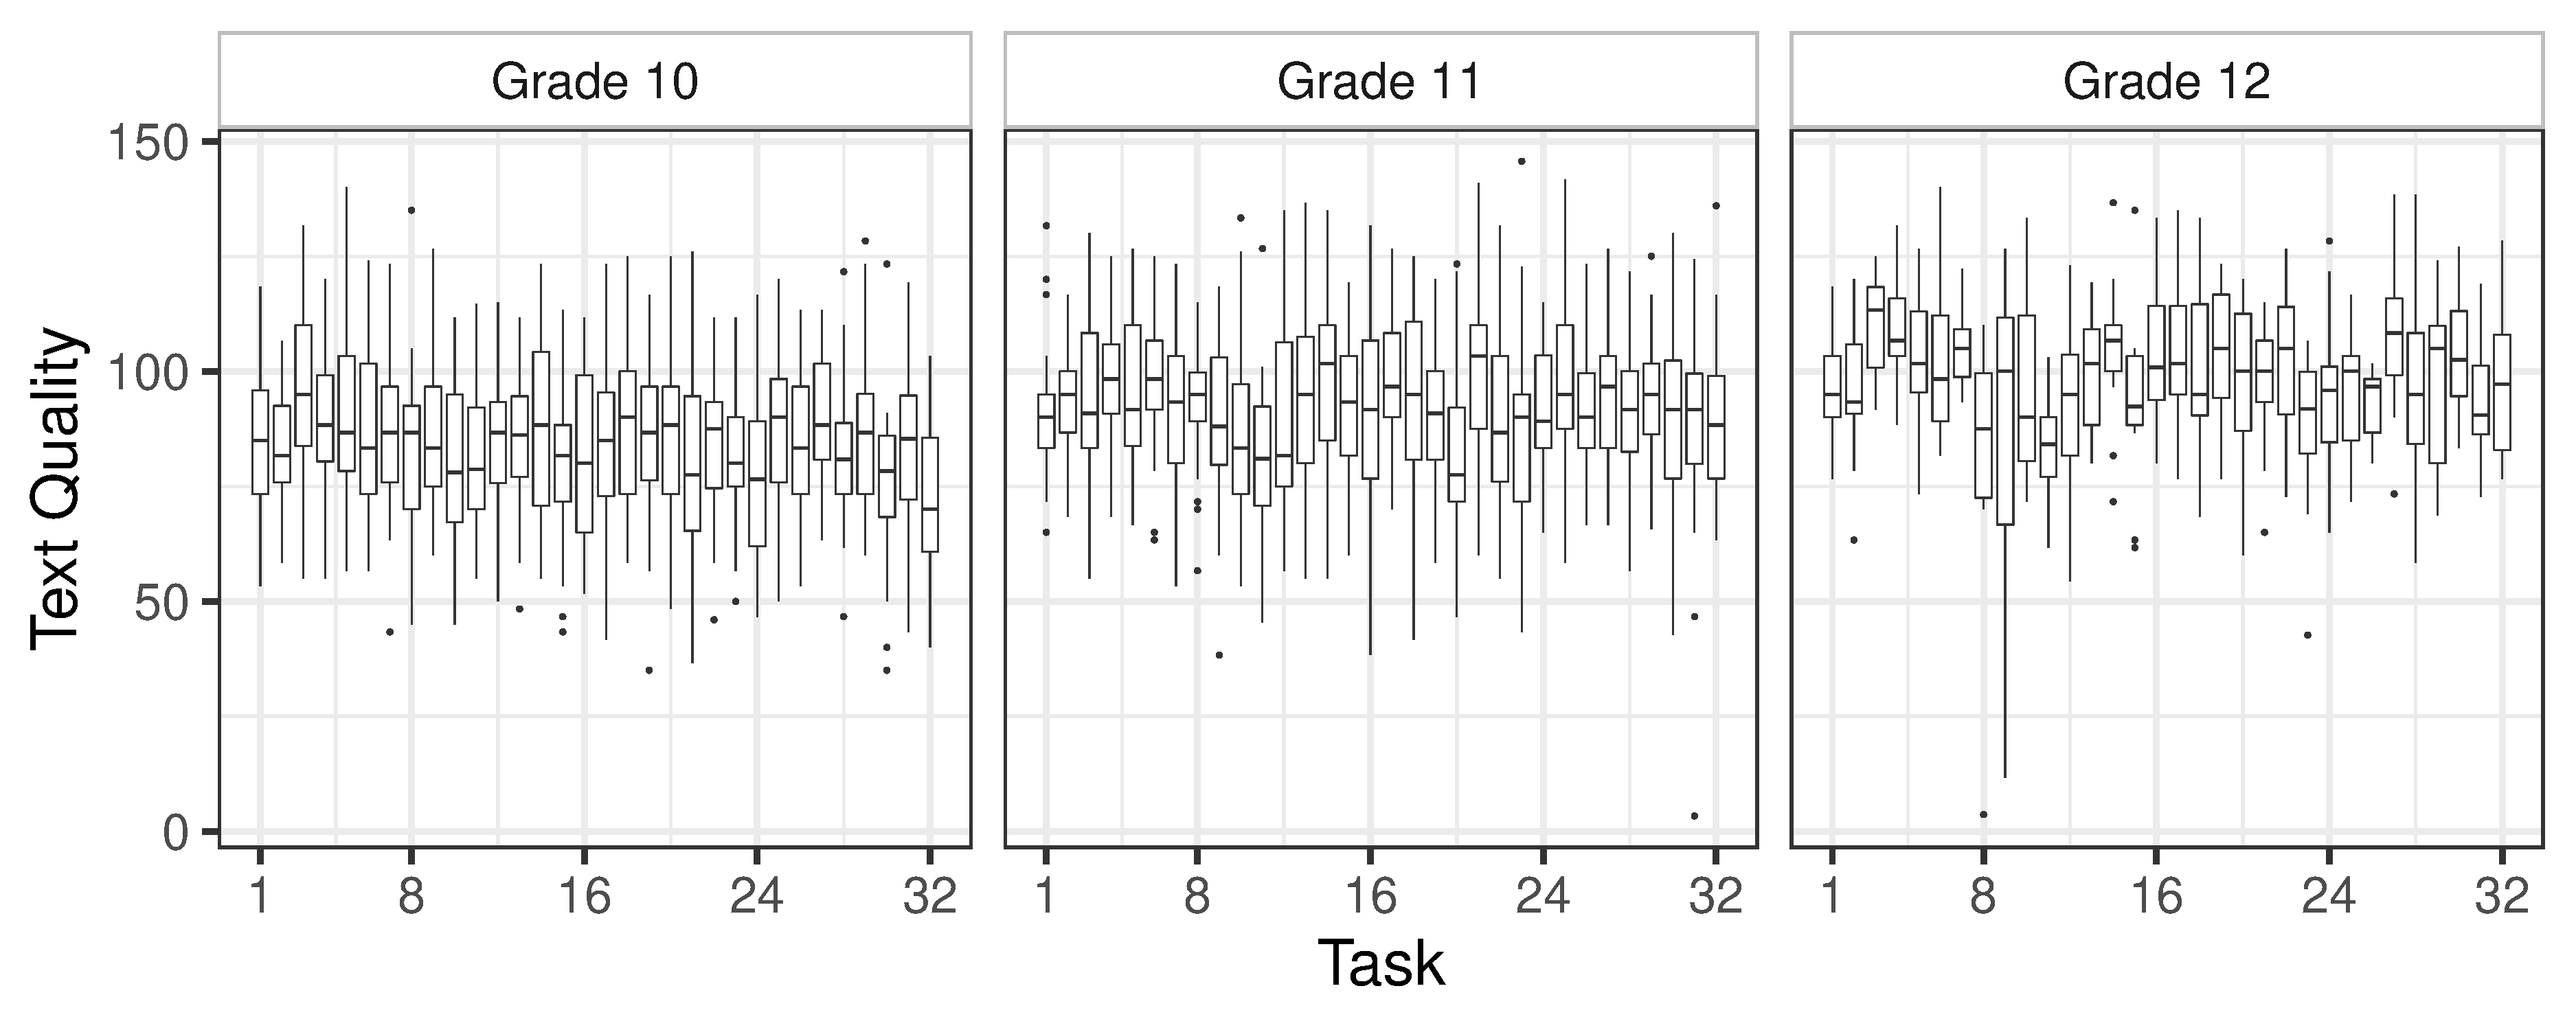
\includegraphics[width=\textwidth]{descriptivesBaseline.pdf}
	\caption{Box and whiskers plot of student performance on each task for the three grades measured. The grade is indicated above each panel and the task code is shown on the x-axis. There is substantial variance in student performance between tasks and within tasks, and student performance appears to increase in successive grades.}
	\label{fig:baselineDescriptives}
\end{figure}
The observations of text quality cannot be considered as independent.
Scores of students in the same school might be more alike than scores of students from different schools.
Likewise, scores on the same task might be more alike than scores on different writing tasks.
Therefore, a cross-classified multilevel model is in operation.
If $y_{(ij)k}$ is the score of student $i$ ($i = 1, 2, 3, ...., I_k$) on task $j$ ($j = 1, 2, ..., J_i$) in school $k$ ($k = 1, 2, ...., K$), we can write the model that we will analyze as a function of student, task, school, and grade:
\begin{align*}
%	y_{(ij)k} = \beta \times \mathrm{Grade}_{ijk} + [w_{00k} + u_{i0k} + v_{0j0} + \epsilon_{(ij)k}].
	y_{(ij)k} &= \beta_0 + \beta_1 \times [\mathrm{Grade}_{(ij)k}=11] + \beta_2 \times [\mathrm{Grade}_{(ij)k}=12]\\
			  &+ w_{00k} + u_{i0k} + v_{0j0} + \epsilon_{(ij)k}.
\end{align*}
The model consists a fixed part, the first line, and a random part, the second line. In the fixed part, $\mathrm{Grade}_{(ij)k}$ is an indicator matrix for students' grade (e.g., for students in grade 11 $[\mathrm{Grade}_{(ij)k}=11] = 1$, otherwise 0). The intercept $\beta_0$ represents the mean writing score in Grade 10. Consequently, the regression weights $\beta_1$ and $\beta_2$ represent the difference in mean writing score between grade 11 and 10, and grade 12 and 10 respectively. In the random part four residual scores are distinguished, all of which are assumed to be normally distributed around with an expected value of 0. The first residual ($w_{00k}$) captures the difference between a school and the average. The second residual ($u_{i0k}$) captures that the average score of student $i$ in school $k$ can deviate from the schools' mean. The third residual ($v_{0j0}$) captures that some tasks might be more difficult than other tasks. The fourth residual ($\epsilon_{(ij)k}$) indicates the deviation of the score of task $j$ of the average of student $i$ in school $k$. Usually, the variance of this term is interpreted as random noise.


\subsection*{Bayesian Inference}
\pgfmathsetmacro{\zCrit}{1.959964}% qnorm(0.975)

This section aims to give a brief introduction to Bayesian inference with an emphasis on the problem at hand. For a more elaborate introduction to Bayesian inference, see the special issue in \emph{Psychonomic Bulletin \& Review} which provides tutorials and guidance for aspiring Bayesians \cite{VandekerckhoveEtAl2018SI}. The choice for a Bayesian analysis is motivated by the fact that Bayesian inference is naturally accompanied by uncertainty estimates, as is explained later. Thus, the estimates of a baseline study and an experimental study can be compared while accounting for the uncertainty in both sets of estimates.

Bayesian inference is centered on the updating of beliefs.
Prior beliefs express our uncertainty about parameter values before observing any data whereas posterior beliefs express our uncertainty about the parameter values after updating the prior beliefs with the observed data.
For any parameter in a given statistical model $\model$, the values this parameter can take are assigned a prior belief.
Beliefs are represented with a probability distribution, usually called the prior distribution for the prior beliefs and posterior distribution for posterior beliefs.
For example, in a multilevel model, the intercept $\beta_0$ can be assigned a normal distribution as prior distribution with mean 0 and variance 1.
Then the a-priori the most likely values for the intercept are near 0 and about 95\% of the prior mass lies within \pgfmathprintnumber{-\zCrit} and \pgfmathprintnumber{\zCrit}.

The key step in Bayesian inference is to use the data $\data$ to update the prior beliefs to posterior beliefs.
The procedure for updating the prior distribution to a posterior distribution is given by Bayes theorem:
\begin{align*}\label{eq:BayesTheorem}
\underbrace{\prob{\bm{\beta} \mid \data , \model}}_{\text{Posterior}}
&=
\overbrace{\prob{\bm{\beta}\mid \model}}^{\text{Prior}}
%\enspace \times %\enspace
\,\,
\underbrace{\overbrace{
		\frac{\lik{\data \mid \bm{\beta}, \model}}{\prob{\data \mid \model}}
	}^{\text{Likelihood}}}_{\substack{\text{Marginal}\\ \text{Likelihood}}}.
\end{align*}
Here, $\bm{\beta}$ represents all parameters in the model. The prior distribution of the parameters is updated through the likelihood of the statistical model. The likelihood is divided by the marginal likelihood so that the posterior distribution is a proper probability distribution (i.e., it integrates to 1). The posterior distribution is key for parameter estimates. For instance, if a single estimate for a parameter is desired, one could use the mean of the posterior distribution. Other often-used point-estimates are the posterior mode and posterior median. Simultaneously with obtaining the posterior, a measure of uncertainty for each parameter is obtained. Since the posterior distribution is a proper probability distribution, we can use it to draw inferences about the parameters. For example, consider the posterior distribution for the intercept, $\prob{\beta_0 \mid \data , \model}$. Questions such as ``Given that we have seen the data, what is the probability that the intercept is larger than 0?'' can be answered by computing $\prob{\beta_0 > 0 \mid \data , \model}$. Likewise, if we find a lower bound $LB$ and upper bound $UB$ for the intercept $\beta_0$ such that $\prob{ LB \leq \beta_0 \leq UB \mid \data , \model} = 0.95$, we can claim: ``Given that we have seen the data, we are $95\%$ confident that the population value of the intercept lies between $LB$ and $UB$.'' This interval is known as the Bayesian $95\%$ credible interval. Another often-used Bayesian uncertainty interval is the 95\% highest posterior density interval (HPD), an interval that contains 95\% of the posterior mass and has the highest probability density.

\subsubsection*{Approximations to Posterior Distributions}
Although Bayes theorem may appear straightforward, in practice the posterior distribution may be a high-dimensional probability distribution that is difficult to study analytically. 
This holds in particular for multi-level models, as the number of dimensions equals the sum of the number of random effects, fixed effects, and variances.
Rather than studying the mathematical form of the posterior, it is easier to simulate random values from the posterior distribution and to use these for inference.
Such simulation methods are commonly referred to as Markov chain Monte Carlo (MCMC).
The idea is that instead of computing a statistic of the posterior distribution in closed form, we draw a large number of random observations from the posterior distribution and use a sample estimator to approximate the statistic of the distribution.
For example, if we are interested in the posterior mean of the intercept, we simulate many observations from the posterior distribution and use the sample mean of these observations to approximate the posterior mean of the intercept.
Likewise, to compute the posterior probability that an intercept $\beta_0$ is positive, $\prob{\beta_0 > 0 \mid \data , \model}$, we take the proportion of MCMC samples where $\beta_0$ is positive.
This procedure is akin to how applied scientists randomly sample participants from a population and then generalize the sample statistics to the population, although with MCMC it is often easy to draw enormous samples to obtain a near-perfect approximation.

%Rather than studying the mathematical form of the posterior, it is much easier to simulate random values from the posterior distribution and to use these for inference. Such simulation methods are commonly referred to as Markov chain Monte Carlo (MCMC). The idea is that instead of computing a statistic of the posterior distribution in closed form, we can draw random observations from the posterior and use a sample estimator to approximate the statistic of the distribution. For example, if we are interested in the posterior mean of the intercept, we simulate many observations from the posterior distribution and use the sample mean of these observations to approximate the posterior mean of the intercept. Likewise, to compute the posterior probability that an intercept $\beta_0$ is positive, $\prob{\beta_0 > 0 \mid \data , \model}$, we examine the proportion of MCMC samples where $\beta_0$ is positive. This procedure is akin to how applied scientists attempt to randomly sample participants from a population and then generalize the sample statistics to the entire population, with the exception that is it relatively easy to draw enormous samples with MCMC to obtain near-perfect approximations.

\subsection*{Statistical Software}
\pgfplotstableread{mcmcSettings.csv}\tbMCMCsettings

All analyses were done in R \cite{R}.
The R package \code{brms} was used for Bayesian multilevel analyses \cite{burkner2017brms}.
The R package \code{brms} is a convenient front-end for the probabilistic programming language Stan, which is software for general-purpose Bayesian inference \cite{carpenter2017stan}.
R code for all analyses is available at \githubLink{}.
For all analyses, we used six MCMC chains to assess convergence.
Convergence was assessed using the $\widehat{R}$ statistic \cite{vehtari2019rank}.
In line with the recommendations by \citeA{vehtari2019rank}, we tweaked the parameters of the Stan algorithm such that the $\widehat{R}$ is less than 1.01 and the rank-normalized effective sample size is larger than 400.
Per chain, we simulated \getValInt{0}{iter}{\tbMCMCsettings} samples and discarded the first \getValInt{0}{warmup}{\tbMCMCsettings} as warmup samples.
In total, results in Tables and Figures are based on \getValInt{0}{total}{\tbMCMCsettings} samples.

We used the default prior distributions of the R package \code{brms} for all parameters. That is, the standard deviations of the random effects and the residual were assigned a half t-distribution with a mean of 0, scale of 18, and 3 degrees of freedom. For the fixed effects we used a Cauchy distribution with location 0 and scale 1.

\section*{Baseline Analysis}

% setup table
\pgfplotstableread{postSummaryBaseline.csv}\tbPostSummaryBaseline

We summarized the posterior distribution in Table~\ref{tb:baselineSummary}.
This shows that the average text quality of students in grade 10 is estimated at \getVal{0}{Mean}{\tbPostSummaryBaseline}.
The 95\% highest posterior density (HPD) credible interval ranges from  \getCI{0}{\tbPostSummaryBaseline}.
Students in grade 11 performed on average about \getVal{1}{Mean}{\tbPostSummaryBaseline} points better (\getCI{1}{\tbPostSummaryBaseline}) than students in grade 10.
Likewise, students in grade 12 performed on average about \getVal{2}{Mean}{\tbPostSummaryBaseline} points better (\getCI{2}{\tbPostSummaryBaseline}) than students in grade 10.
However, the estimated variance between schools (\getVal{3}{Mean}{\tbPostSummaryBaseline}), students within school (\getVal{4}{Mean}{\tbPostSummaryBaseline}), and tasks (\getVal{5}{Mean}{\tbPostSummaryBaseline}) clearly deviate from 0.
Since the data set contained such a large variety of schools and tasks, these findings likely generalize over tasks.
\begin{table}[!ht]
	\caption{Summary of the posterior distribution for the baseline data set. The first column shows the parameter, the second the posterior mean for that parameter, the third the posterior standard deviation and the last two columns show the 95\% higher posterior density interval. Grade 11 and 12 represent the improvement relative to grade 10 (the intercept).}
	\label{tb:baselineSummary}
	\centering
	\pgfplotstabletypeset[
	column type=r,
	every head row/.style={
		before row={
			\toprule
			\multicolumn{1}{c}{} & \multicolumn{1}{c}{} & \multicolumn{1}{c}{} & \multicolumn{2}{c}{95\% HPD} \\
			\cmidrule[0.4pt]{4-5}
		},
		after row=\midrule,
	},
	every last row/.style={
		after row=\bottomrule
	},
	columns/Parameter/.style={string type}
	]\tbPostSummaryBaseline
\end{table}

Figure~\ref{fig:baselinePosteriorTextQuality} visualizes the improvement in text quality across grades. To obtain the posterior distributions for grades 11 and 12, we add the posterior distribution of the intercept to that of the improvement in Grade 11 and Grade 12.
\begin{figure}[!ht]
	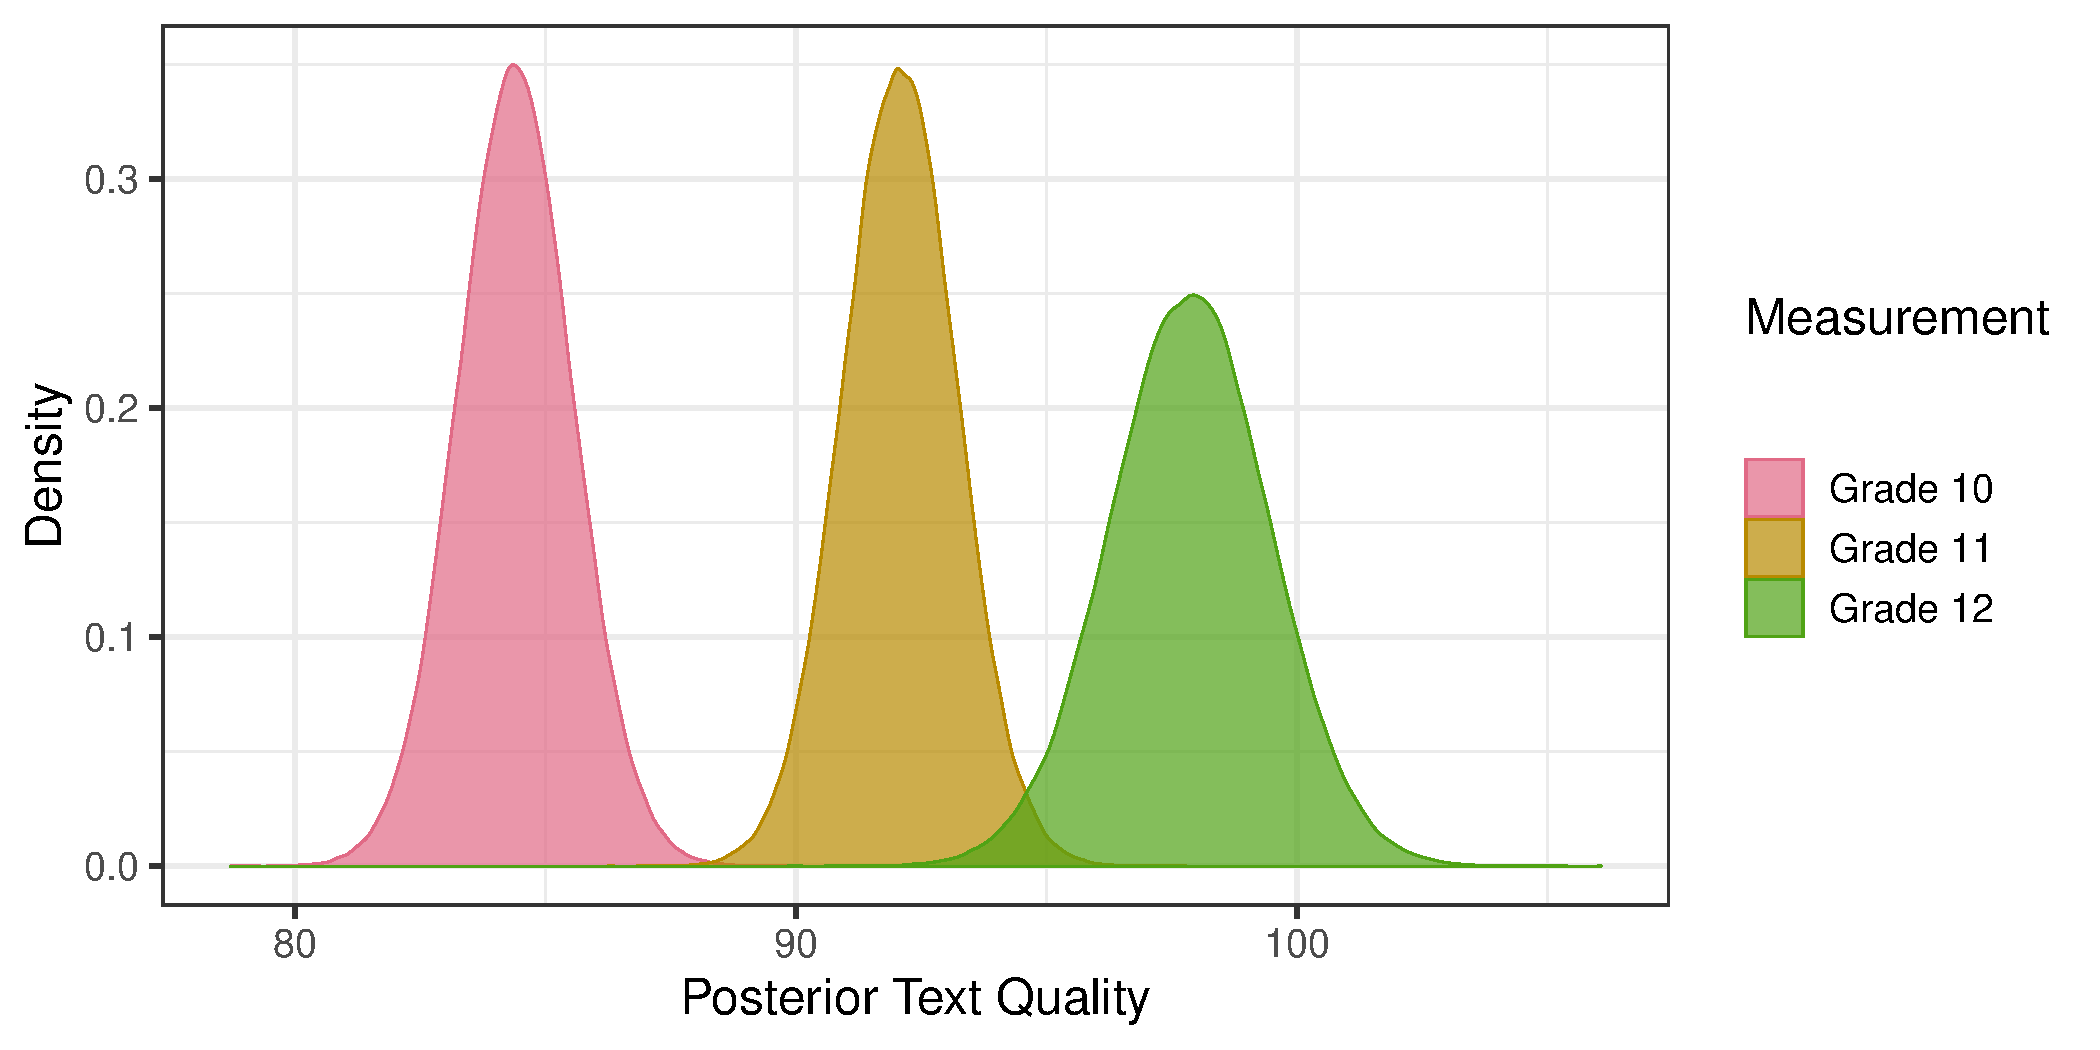
\includegraphics[width=\textwidth]{posteriorTextQualityBaseline}
	\caption{Posterior distribution of text quality in grades 10, 11, and 12. Posteriors distributions for grades 11 and 12 are obtained by adding the MCMC samples of the intercept to the MCMC samples for the improvement of the respective grade.}
	\label{fig:baselinePosteriorTextQuality}
\end{figure}

The descriptive plot in Figure~\ref{fig:baselineDescriptives} suggested that the scores of students depend on the task they made. This is further confirmed by the posterior mean of between task variance \getVal{5}{Mean}{\tbPostSummaryBaseline} (\getCI{5}{\tbPostSummaryBaseline})) which is far away from 0. This shows that differences between tasks are substantial and that some tasks are systematically more difficult than others. Thus, the mean score of students depends on the task they take.

\section*{Application to an Experimental Analysis}

\subsection*{Data Set}
Data were collected from 89 students of two high-schools in the Netherlands.
Students made three writing tasks in one week; one on Monday, Wednesday, and Friday.
Prior to writing the second and third text, the participants received feedback on their previously written text.
As part of the feedback, students received annotated exemplar texts selected from the national baseline; these are texts that are representative for a specific position on the benchmark scale, accompanied with a description for several text quality aspects.
Students could compare and contrast their own text with the exemplar texts of students with the same or a better score.

\begin{figure}[!ht]
	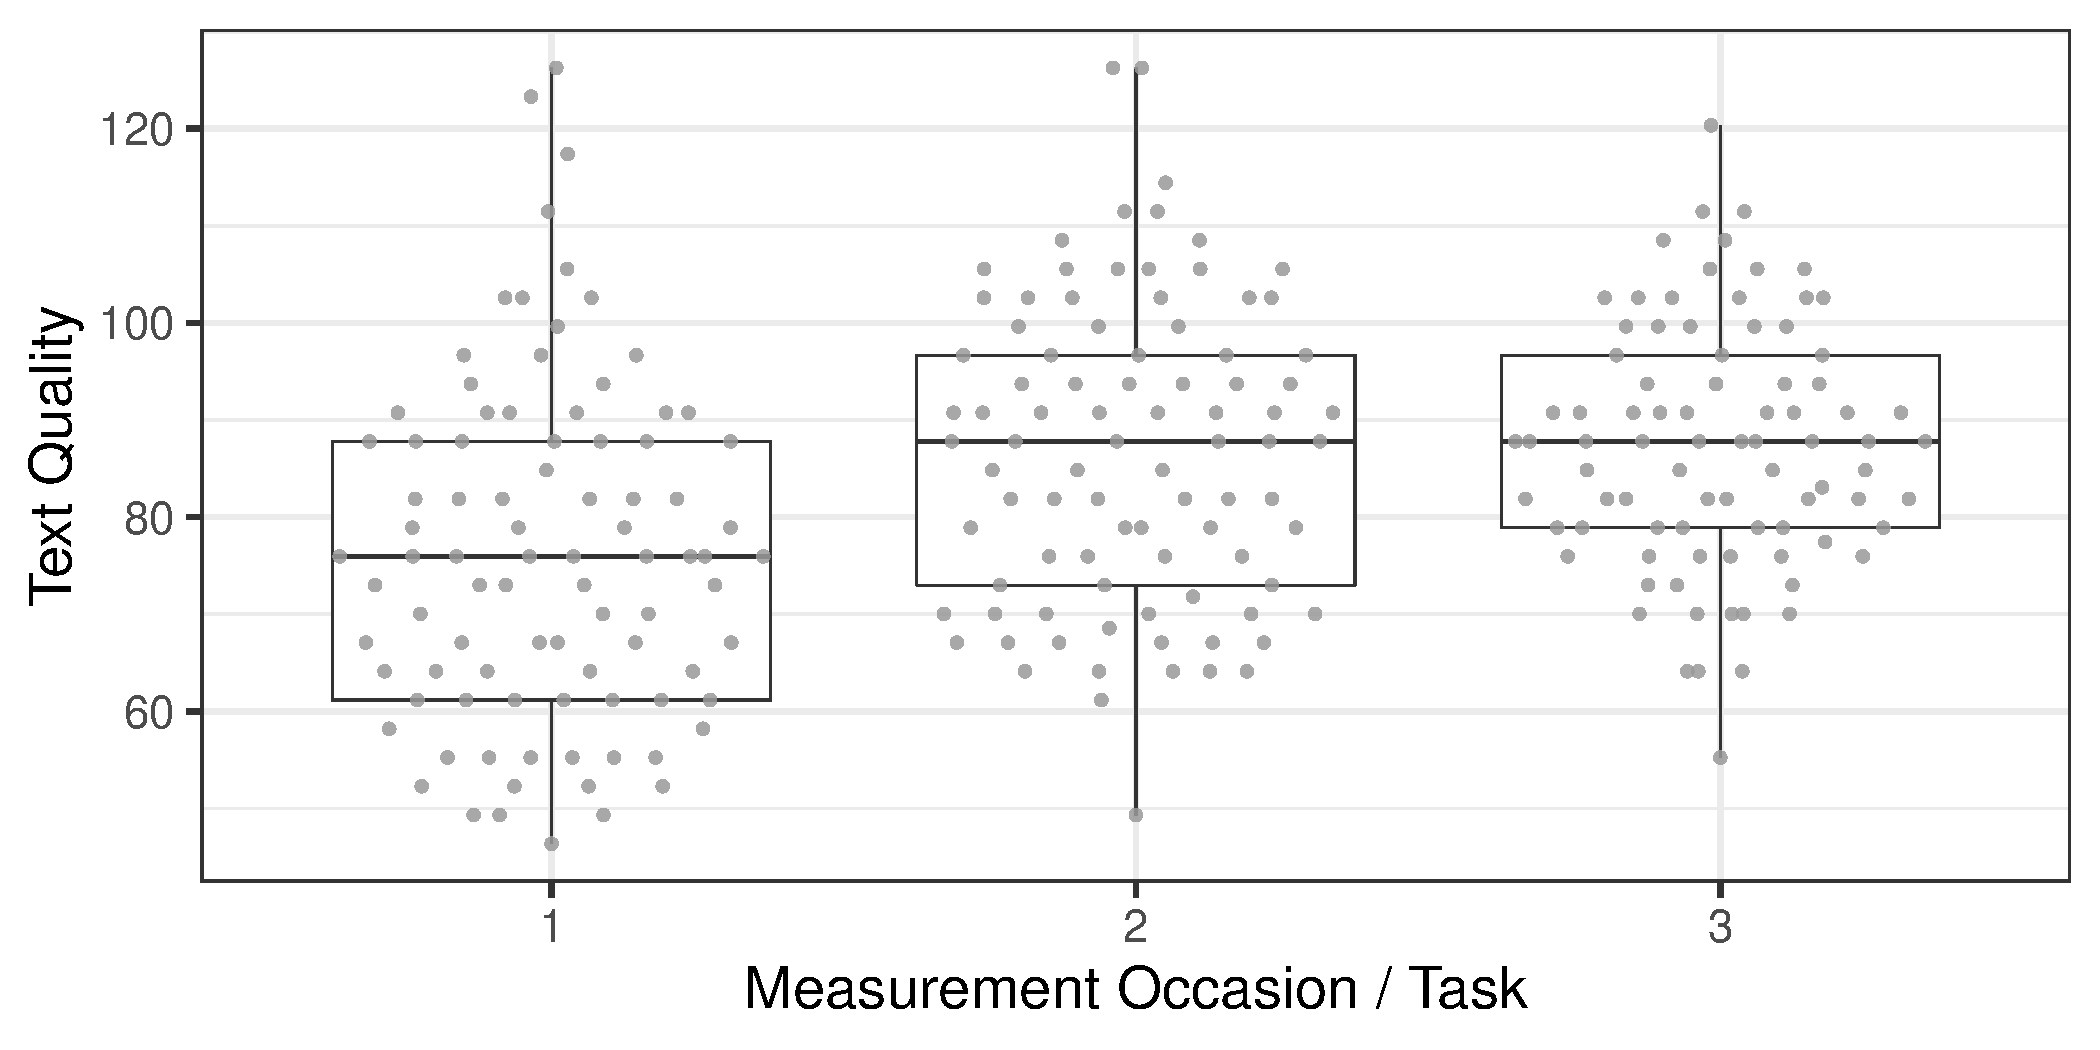
\includegraphics[width=\textwidth]{descriptivesExperimental}
	\caption{Box and whiskers plot of student performance on the three measurement occasions. Grey points represent the raw scores on text quality. Quasi-random jitter was added to the x-coordinates of the points to avoid visual clutter. The average performance clearly increases from measurement one to two, but it is hard to quantify the improvement without a reference group.}
	\label{fig:productDescriptives}
\end{figure}

\subsection*{Analysis}
\pgfplotstableread{postSummaryExperimental.csv}\tbPostSummaryProduct

A typical analysis for this data set is almost identical to that of the baseline data set, except that here we estimate differences between measurements, which might be contaminated with differences due to tasks. Since each student took only one task at each measurement occasion, the between-task variance cannot be estimated. Thus $y_{hik}$ is the observation of measurement $h$ ($h=1, 2, 3$) of student $i$ ($i=1, ..., K_i$) in school $k$ ($k = 1, 2$). The multilevel model thus becomes:
\begin{align*}
%y_{(ij)k} = \beta_0 + \beta \times \mathrm{Measurement}_{ijk} +  [w_{00k} + u_{i0k} + \epsilon_{ijk}].
y_{hik} &= \beta_0 + \beta_1 \times [\mathrm{Measurement}_{hik} = 2] + \beta_2 \times [\mathrm{Measurement}_{hik} = 3]\\
        &+ w_{00k} + u_{0ik} + \epsilon_{hik}.
\end{align*}
%Here, $y_{hjk}$ is the observation of student $i$ on measurement $j$ in school $k$. 
The fixed part consists of an intercept ($\beta_0$) that represents the mean writing score on the first measurement and two fixed effects that capture the difference in mean writing score between subsequent measurements and the first measurement ($\beta_1$ and $\beta_2$).
The random part consists of a random intercept for school ($w_{00k}$), a random intercept for person within school $u_{i0k}$ and a residual $\epsilon_{hik}$.
%\begin{align*}
%y_{psm} &= \beta_0 + \beta_p + \beta_s + \beta_m  + \epsilon_{pstg}.
%\end{align*}
%Here, the observation of student $p$ in school $s$ on measurement $m$ is denoted $y_{psm}$. The score consists of an intercept $\beta_0$, a random intercept for person $\beta_p$ and school $\beta_s$, and a fixed effect of measurement $\beta_m$.
As for the baseline analysis, we summarize the posterior distribution of the multilevel model using the mean, standard deviation, and HPD in Table~\ref{tb:productPosteriorSummary}. This shows that the average text quality is estimated at \getVal{0}{Mean}{\tbPostSummaryProduct} (\getCI{0}{\tbPostSummaryProduct}). At the second measurement occasion, students performed on average about \getVal{1}{Mean}{\tbPostSummaryProduct} points better (\getCI{1}{\tbPostSummaryProduct}) than at intake. At follow up, students' improvement was estimated at \getVal{2}{Mean}{\tbPostSummaryProduct} (\getCI{2}{\tbPostSummaryProduct}). A bivariate scatterplot for the parameters in Table~\ref{tb:productPosteriorSummary} is shown in Figure~\ref{fig:productPosteriorDescriptives}.

\begin{table}[!ht]
	\caption{Summary of the posterior distribution for the experimental data set. The first column shows the parameter, the second the posterior mean for that parameter, the third the posterior standard deviation and the last two columns show the 95\% higher posterior density interval. The improvement of measurement 2 and 3 is relative to the intercept (measurement 1).}
	\label{tb:productPosteriorSummary}
	\centering
	\pgfplotstabletypeset[
		column type=r,
		every head row/.style={
			before row={
				\toprule
				\multicolumn{1}{c}{} & \multicolumn{1}{c}{} & \multicolumn{1}{c}{} & \multicolumn{2}{c}{95\% HPD} \\
				\cmidrule[0.4pt]{4-5}
			},
			after row=\midrule,
		},
		every last row/.style={
			after row=\bottomrule
		},
		columns/Parameter/.style={string type}
	]\tbPostSummaryProduct
\end{table}

The estimated improvement across measurement occasions is shown in Figure~\ref{fig:productPosteriorTextQual}. Apparent is that students perform better at post-test than at pre-test and that the difference between follow up and post-test appears negligible.
\begin{figure}[!ht]
	\centering
	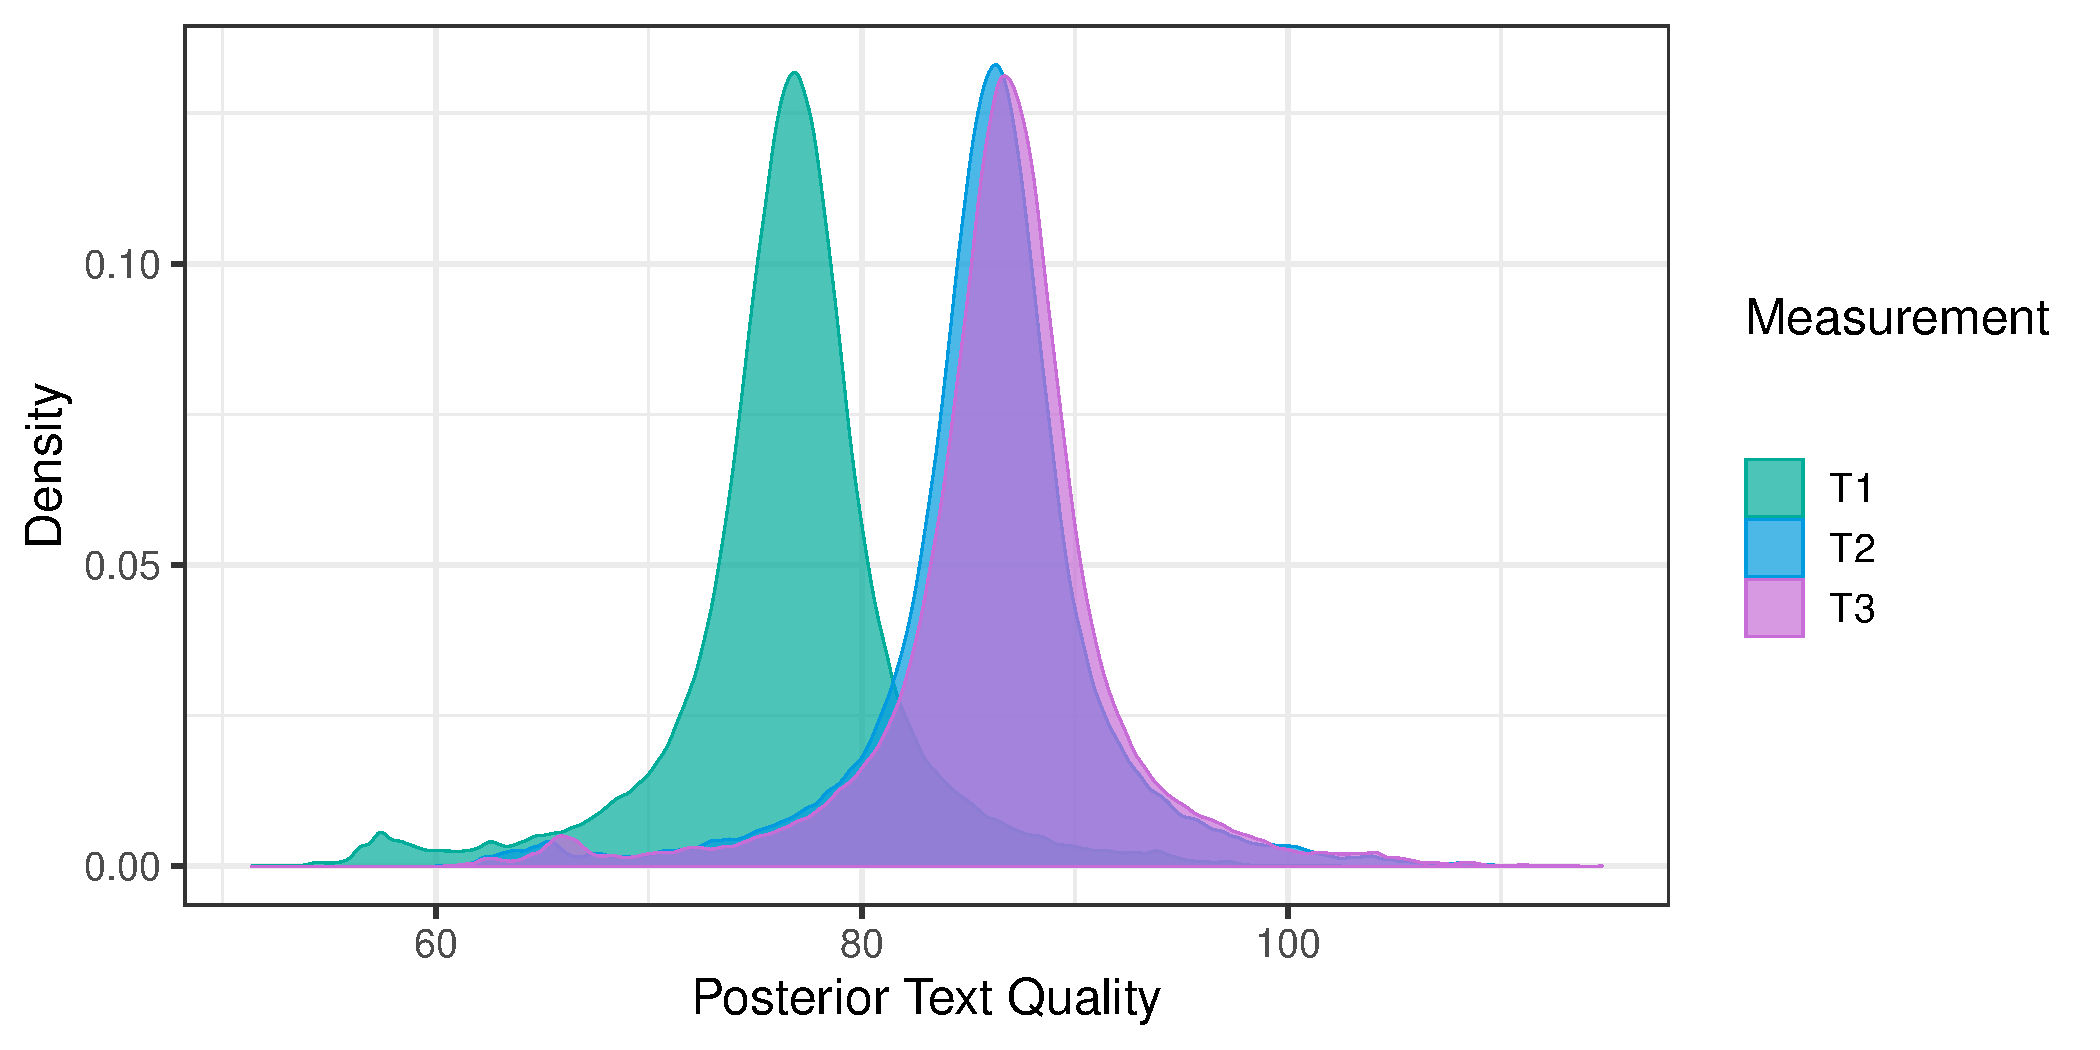
\includegraphics[width=\textwidth]{posteriorTextQualityExperimental.pdf}
	\caption{Posterior distribution of text quality at each measurement occasion of the product data set.}
	\label{fig:productPosteriorTextQual}
\end{figure}
At this point in the analysis, drawing conclusions about the effect of the treatment is problematic because there is no control group. Thus, the improvement of the students cannot solely be attributed to just the intervention but might be caused by differences in difficulty between tasks.
%Thus, it is difficult to interpret the improvement of the students over the measurement occasions, as variation in the students' performance may be caused by between task variance. Given the


%\subsection*{Relating Baseline Result to Experimental Findings}
\subsection*{Relating Baseline Results to the Analysis of an Experimental Study}
\pgfplotstableread{postMeansCorrectedExperimental.csv}\tbPostMeansProdCC

Ideally, we directly compare the difference in text quality between measurement occasions in the experimental study. However, interpreting these differences is not straightforward as the contamination of task effect and measurement occasion makes this impossible. To make the differences between measurement occasions interpretable we need to correct these for task difficulty. As the baseline study provides estimates of task difficulty, a correction is self-evident.  We can correct students' scores in the experimental study by subtracting the estimated task in the baseline study. As a consequence, the corrected posterior means for each measurement occasion changed slightly, see Figure~\ref{fig:comparePostTextQual} (from \getVal{0}{Mean}{\tbPostMeansProdCC} to \getVal{3}{Mean}{\tbPostMeansProdCC} for measurement 1, from \getVal{1}{Mean}{\tbPostMeansProdCC} to \getVal{4}{Mean}{\tbPostMeansProdCC} for measurement 2, and from \getVal{2}{Mean}{\tbPostMeansProdCC} to \getVal{5}{Mean}{\tbPostMeansProdCC} for measurement 3). Note that a direct comparison is possible because the rating procedure of the experimental study is based on the rating procedure of the baseline study.
\begin{figure}[!ht]
	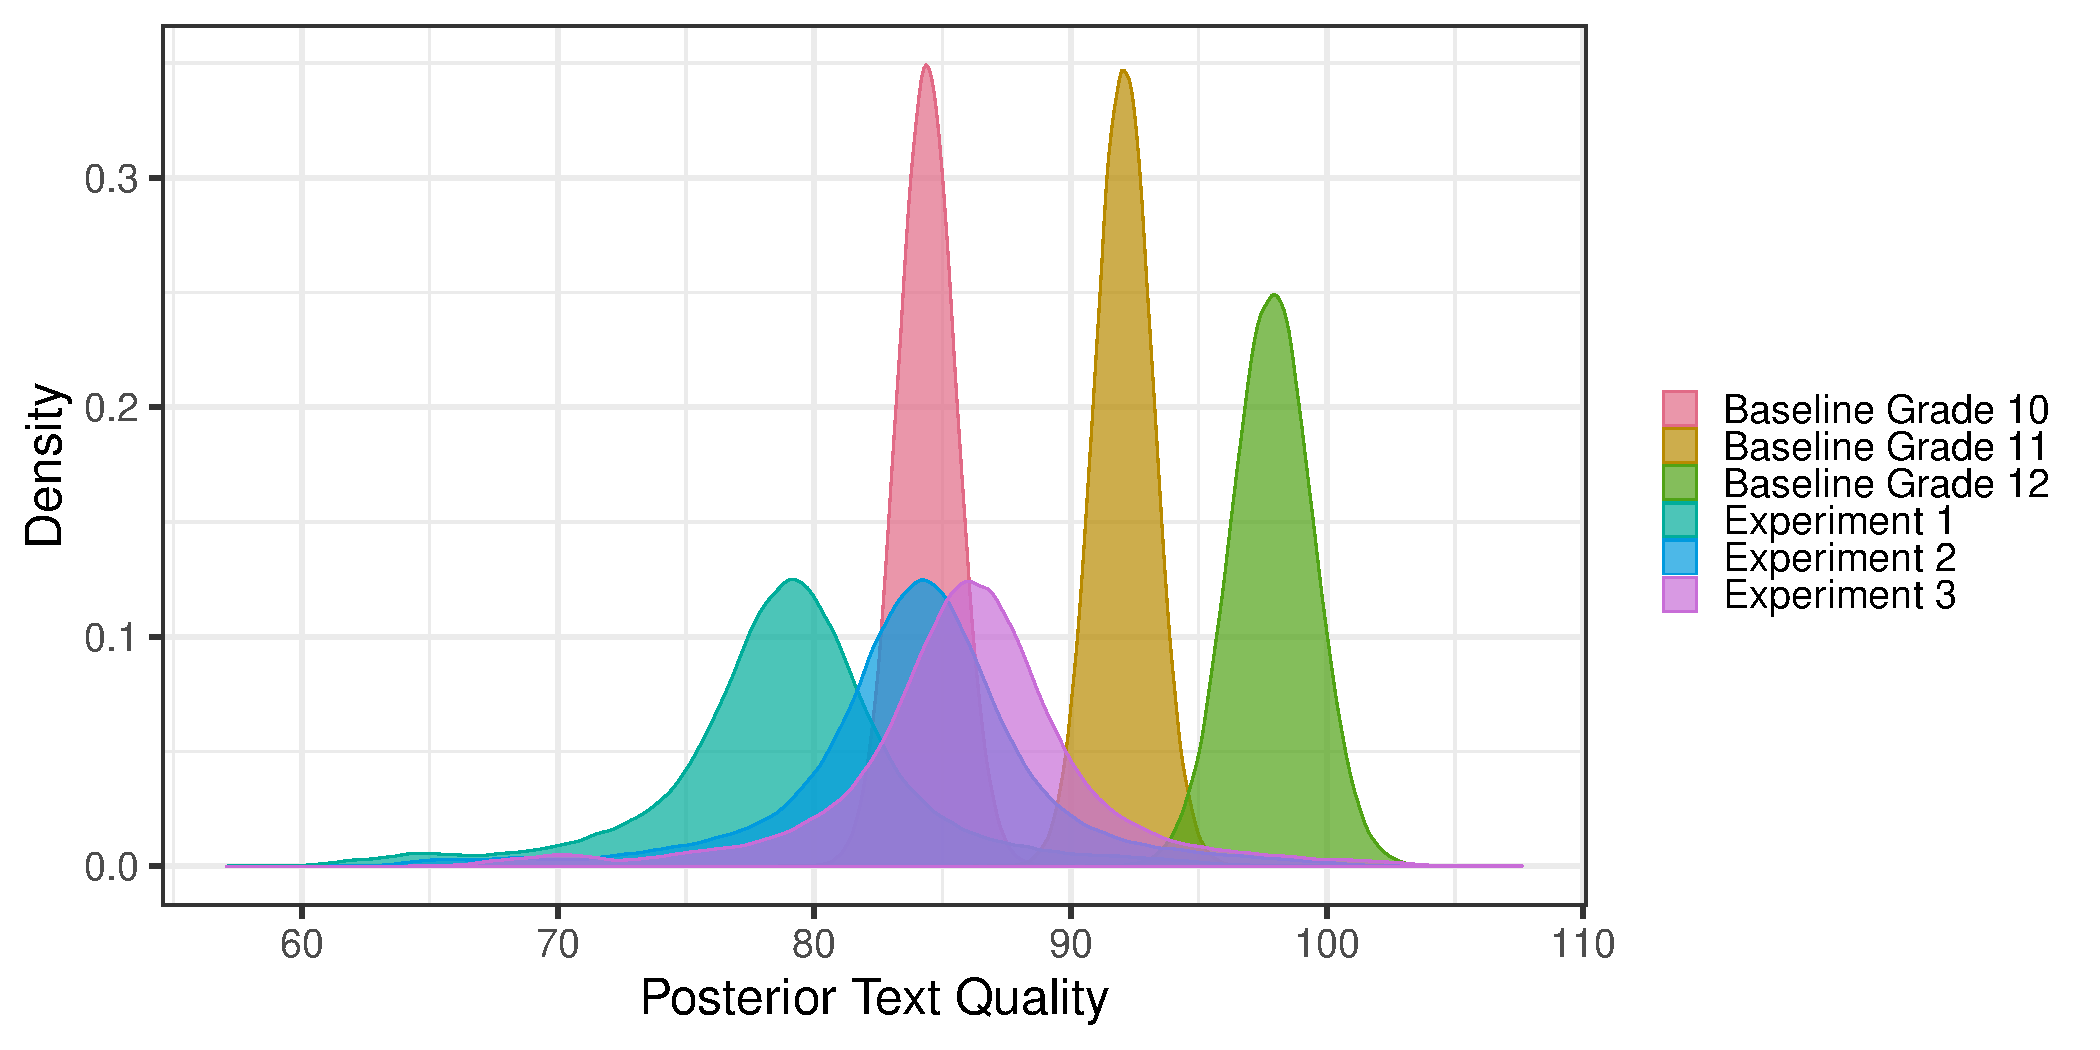
\includegraphics[width=\textwidth]{comparePosteriorTextQuality.pdf}
	\caption{Posterior distributions for each grade in the baseline study and each measurement occasion in the experimental study. The posterior distributions of the baseline study are more narrow because they are based on more observations. We subtracted the estimated average task effect of each task category in the baseline study from the posteriors distributions in the experimental study to correct these for task effect.}
	\label{fig:comparePostTextQual}
\end{figure}

From Figure~\ref{fig:comparePostTextQual} we can infer that the corrected difference between measurement 1 and measurement 2 in the experimental study is almost as large as the difference between grade 10 and 11 in the baseline study. Hence, there is a substantial difference between both measurements and thus an effect. By comparison, the difference between measurement 2 and measurement 3 is much smaller. Of course, this is not a statistical test of significance. Typically, such a test should account for between-task variance. To obtain an estimate for the magnitude of between-task effects we can use the estimates of the baseline study to simulate a distribution of task difficulty. Next, we can compute the probability that the observed difference between measurement occasions in the experimental study is due to differences between tasks.

Since multilevel models typically assume that the random effects follow a normal distribution with mean 0 we simulate a large number these from a normal distribution. As variance, we use the posterior samples for the between-task variance, to propagate the uncertainty in this parameter into the distribution over task-effects.\footnote{Essentially, the effects of these new random tasks are drawn from the posterior predictive distribution of the baseline study.} In total \getValInt{0}{total}{\tbMCMCsettings} task-effects were sampled (the same amount as MCMC samples). Next, we can visualize the posterior distribution of improvement between measurement occasions and contrast this to the distribution over task-effects, as shown in Figure~\ref{fig:posteriorImprovement}.
\begin{figure}[!ht]
	\centering
%	\begin{subfigure}{.33\textwidth}
%		\centering
%		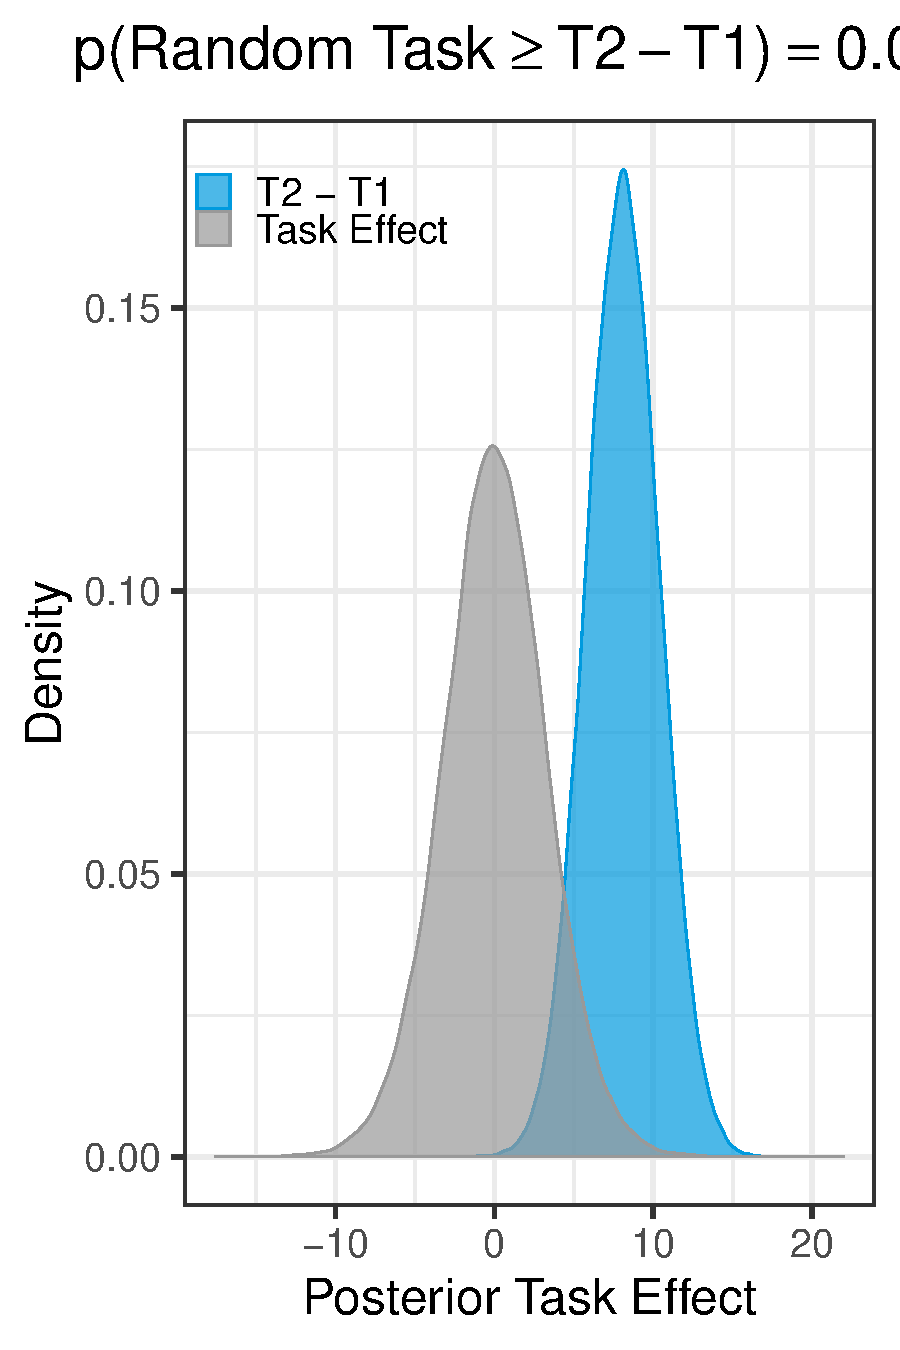
\includegraphics[width=\linewidth]{compareTaskEffectToT2.pdf}
%	\end{subfigure}%
%	\begin{subfigure}{.33\textwidth}
%		\centering
%		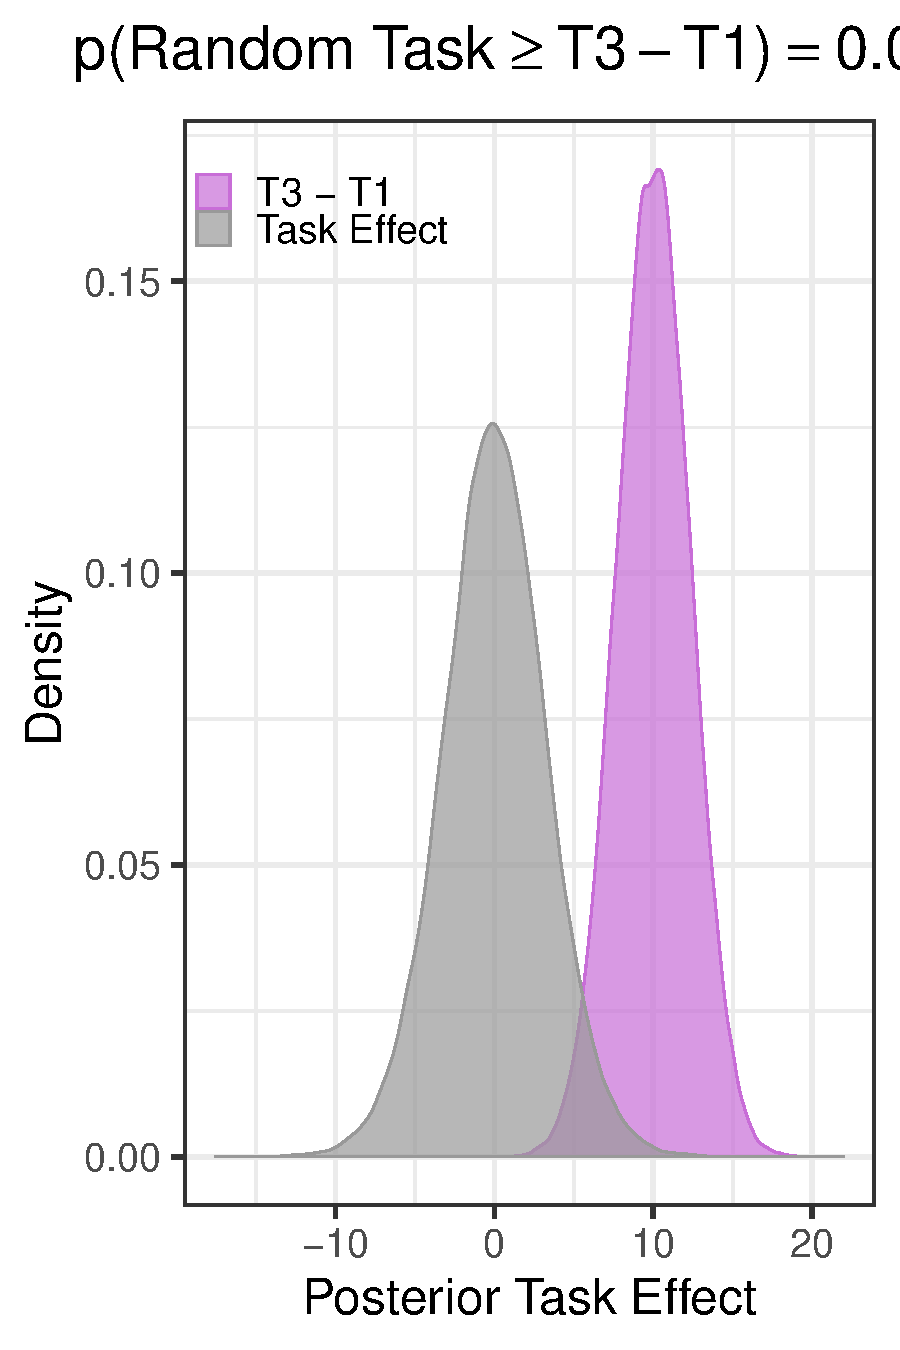
\includegraphics[width=\linewidth]{compareTaskEffectToT3.pdf}
%	\end{subfigure}%
%	\begin{subfigure}{.33\textwidth}
%		\centering
%		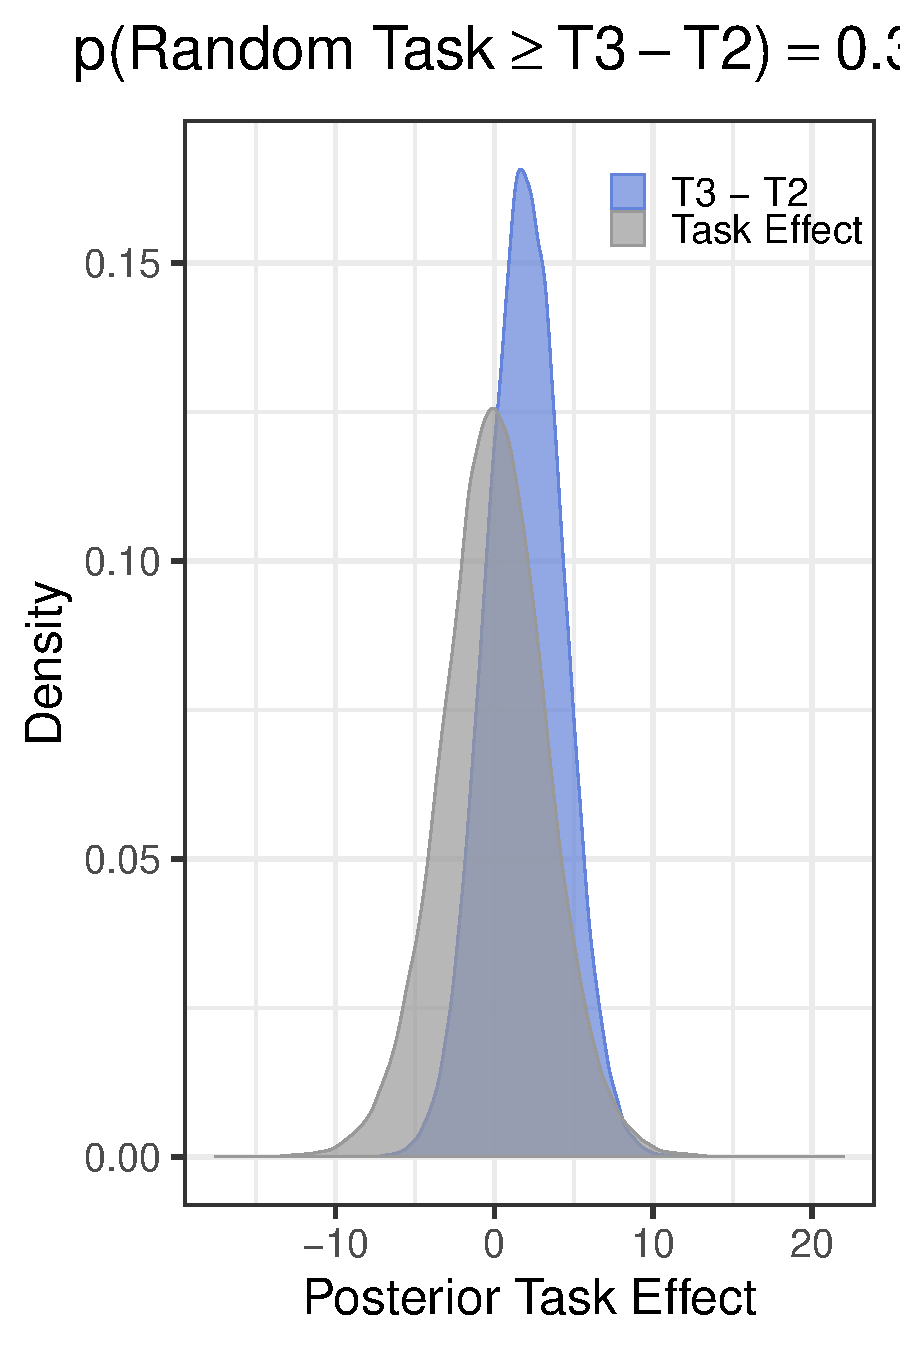
\includegraphics[width=\linewidth]{compareTaskEffectToT23.pdf}
%	\end{subfigure}%
	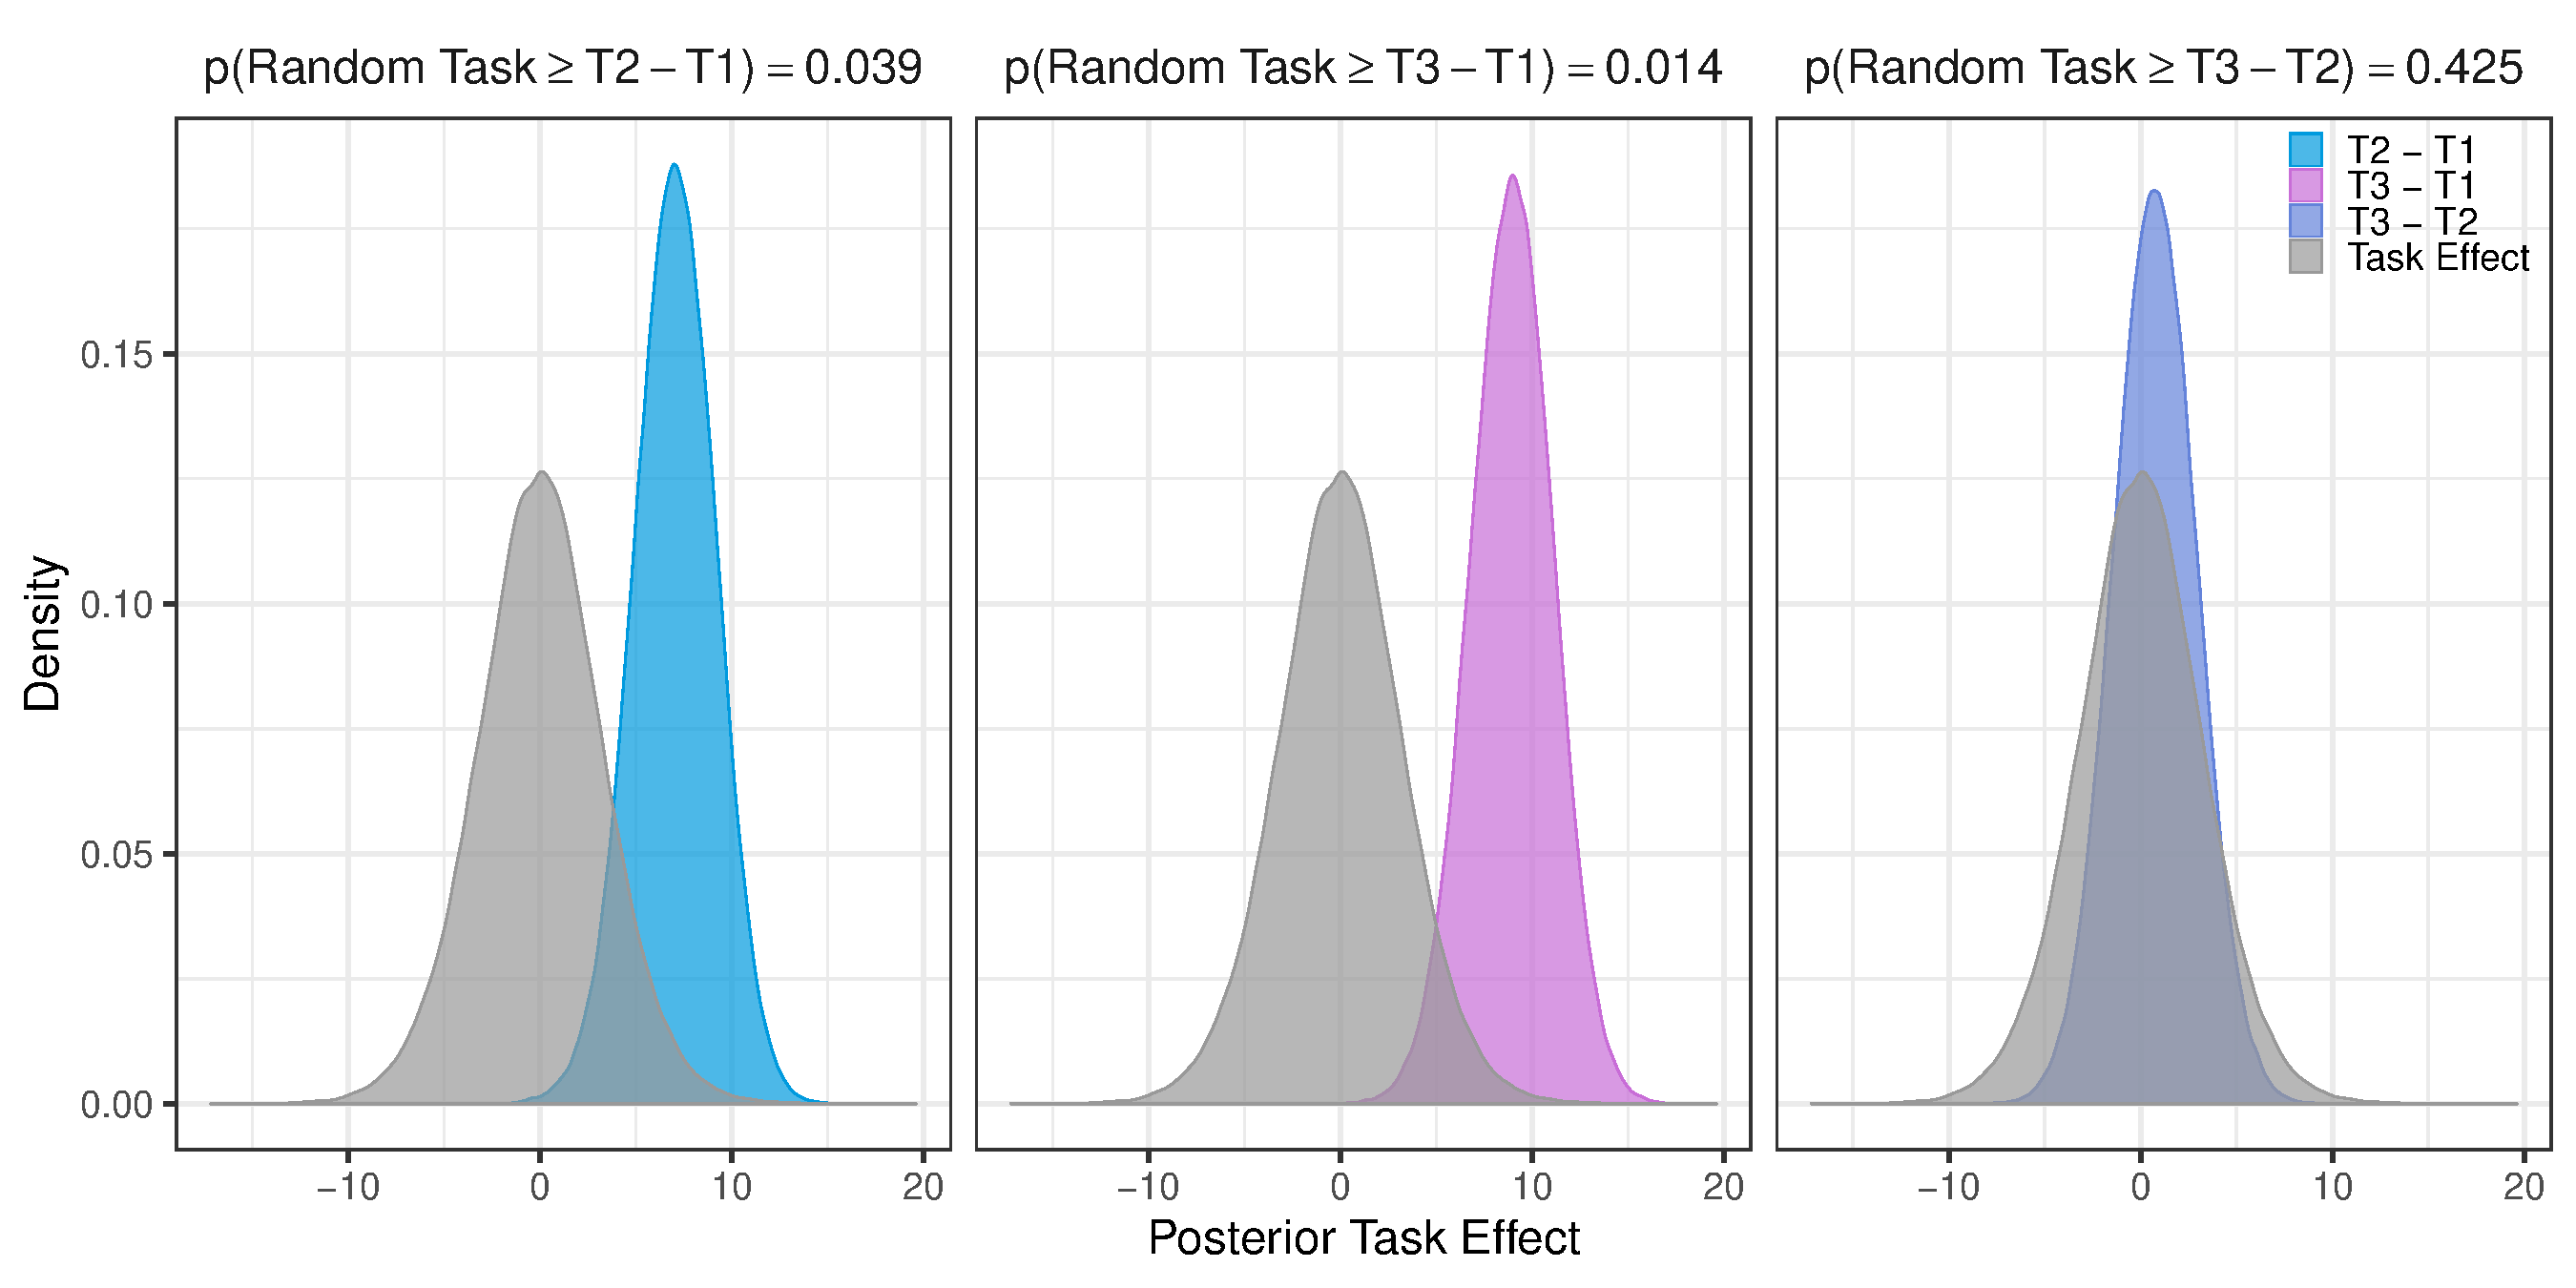
\includegraphics[width=\textwidth]{compareTaskEffects.pdf}
	\caption{Distribution of the effect of a random task (grey) versus the posterior distribution of the estimated progress in the experimental data. The blue density in the left panel is the posterior distribution of improvement between the first and second measurement; the purple density in the middle panel is the posterior distribution of improvement between the first and third measurement; the dark blue density in the right panel is the posterior distribution of improvement between the second and third measurement. The probability that a random task is larger than the improvement is shown above each panel.}
	\label{fig:posteriorImprovement}
\end{figure}

The left and middle panel in Figure~\ref{fig:posteriorImprovement} contrast measurement occasions 2 and 3 against intake.
The improvement appears to exceeds what would be expected of a random task-effect.
The right panel contrasts measurement 2 with measurement 3. Here, the improvement seems indistinguishable from a random task-effect.
This makes sense as there was no intervention between measurements 2 and 3.
\GR{``There WAS an intervention between 2 and 3.''\\ Don: Wat was deze interventie? Wat zal ik hierover schrijven?}


The above results show that the observed effect between measurement occasions 1 and 2 is greater than can be expected from any given task.
However, this does not provide a straightforward manner to interpret the magnitude of this effect.
To obtain a measure that is easy to interpret, we again compare the results to that of the baseline.
From the baseline study, we obtained a posterior distribution that quantifies students' improvement between grade 10 and grade 11, accounting for differences between tasks (i.e., parameter Grade 11 in Table~\ref{tb:baselineSummary}).
Next, we take the posterior samples for the effect of measurement in the experimental study (Parameter Measurement 2 in Table~\ref{tb:productPosteriorSummary}) and divide these by the samples of the baseline study.
The resulting posterior distribution expresses the progress of students in the experimental study in baseline study years and provides a practically intuitive interpretation for the effect size.
The resulting posterior distributions are shown in Figure~\ref{fig:improvementInYears}.

% these cannot be generated inside the caption
\pgfplotstableread{credibleIntervalsImprovementAllYears.csv}\tbCRIimprovement
\setVal{0}{Lower}{\tbCRIimprovement}{\criLowerA}
\setVal{0}{Upper}{\tbCRIimprovement}{\criUpperA}
\setVal{1}{Lower}{\tbCRIimprovement}{\criLowerB}
\setVal{1}{Upper}{\tbCRIimprovement}{\criUpperB}
\setVal{2}{Lower}{\tbCRIimprovement}{\criLowerC}
\setVal{2}{Upper}{\tbCRIimprovement}{\criUpperC}
\begin{figure}[!ht]
	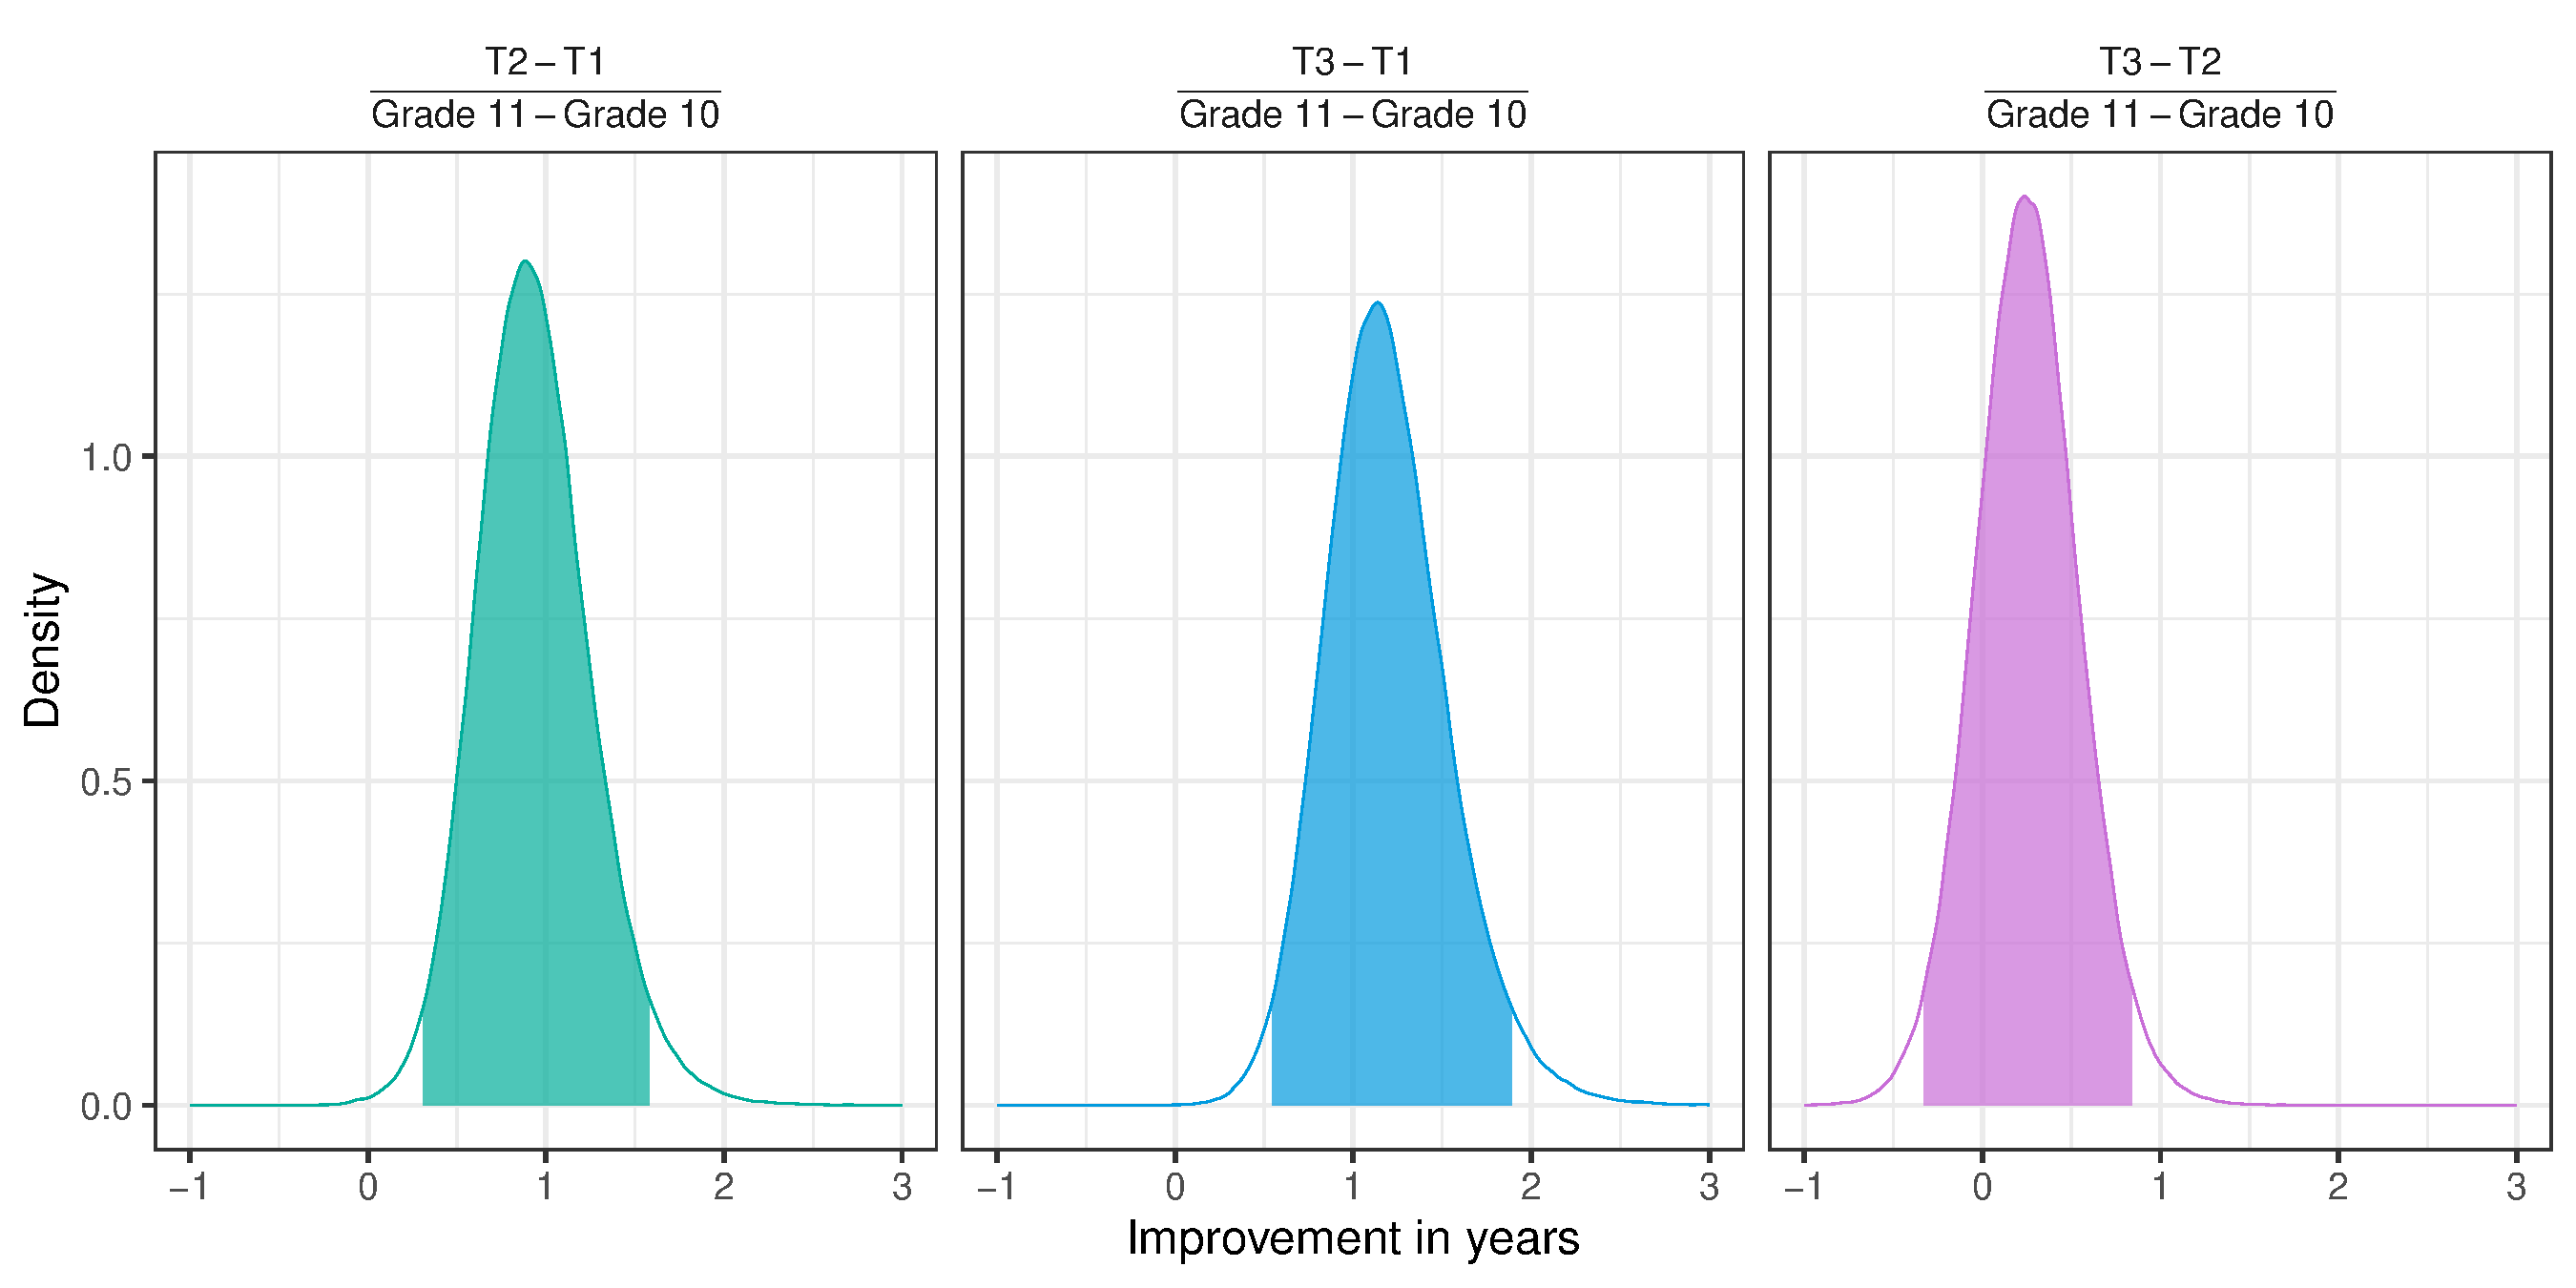
\includegraphics[width=\textwidth]{improvementInAllYears.pdf}
	\caption{Improvement in the experimental study relative to the improvement between grade 11 and grade 10. The left panel shows the posterior distribution for the improvement between measurement 1 and measurement 2 divided by the improvement from grade 10 to 11 (95\% HPD [$\criLowerA$, $\criUpperA$]). The middle panel shows the improvement from measurement 1 to measurement 3, standardized in the same manner (95\% HPD [$\criLowerB$, $\criUpperB$]). The right panel shows the improvement between measurement 2 and 3  (95\% HPD [$\criLowerC$, $\criUpperC$]). The shaded areas under the curve represent 95\% HPD intervals.}
	\label{fig:improvementInYears}
\end{figure}

In the left panel of Figure~\ref{fig:improvementInYears}, the posterior has a mean \getVal{0}{mean}{\tbCRIimprovement} (\getCI{0}{\tbCRIimprovement}), which indicates that the students appear to have gained almost a year in ability between the two measurements. In the middle panel, the posterior mean is \getVal{1}{mean}{\tbCRIimprovement} (\getCI{1}{\tbCRIimprovement}) which indicates that this improvement is still present at the third measurement. In the rightmost panel, the mean improvement is \getVal{2}{mean}{\tbCRIimprovement} (\getCI{2}{\tbCRIimprovement}) which is much smaller and indicates less improvement between measurement occasions two and three.


\section*{Discussion}
%\DONa{verwerkt dit comment in de discussie: om didactische redenen lijkt het me idd goed om het onderscheid tussen de experimenten er avn buiten te laten, maar aan het eind zou het een mooi sluitstuk zijn als je wel laat zien hoe je dan met twee xperimentele condities kunt werken. Voordeel van de beshcikking van een baseline is dat je niet een controlegroep hoeft mee te nemen, maar dat je tijd en geld kunt besteden aan een theoretisch interessante experimentele tegenhanger.}

In this paper, we related the results of an experimental study to those of a baseline study.
The post-intervention improvement in the experimental study exceeded the differences between random tasks in the baseline study.
Therefore, we interpret the effect of the intervention as significant.
We further quantified this effect by expressing the improvement in the number of school years.



%\DON{1. Samenvatten effect van interventie aangetoond door vergelijking met baseline 2. generaliseerbaarheid over taken. 3. wat er nu staat.}
%In this paper, we introduced a procedure for comparing results from a large scale assessment into the analysis of an experimental study that lacked a control group.
%\GRa{Maar is dat het probeem? Het probleem is dat de vooruitgang van T1 naar T2 gecontamineerd is met taak. Een controlegroep zou daar wel iets aan kunnen helpen, maar ook in die groep kan helden dat T2 veel makkelijker/moeilijker zou kunnen zijn.  De crux likt mij dat je op deze manier de scores op T1 en T2 zuivert voor taakeffecten, en dus het vershcil tussen T1 en T2 beter te interpreteren is. Don: dat is een heel extreem standpunt.}

If a control group is missing, the task-effect cannot be disentangled from the effect of an intervention.
However, by relating the increase in performance to estimates of the between-task variance in a baseline study, we can compute how probable it is that improvement across measurements is a task-effect.
This method could provide a point of reference for studies without a control group and may help discern between statistically significant effects and practically relevant effects \cite{hojat2004visitor, fan2001statistical}.

A comparison with a baseline study can also enrich the results of studies with a control group.
For example, if a study administers a smaller variety of tasks than a baseline study, a comparison can provide a clearer assessment of the generalization of an effect over tasks.

Comparing the distribution of task-effect in an experimental study to that of a baseline study relates to approaches of statistical tests for equivalence, such as TOST \cite{lakens2017equivalence}, ROPE \cite{kruschke2011bayesian}, and interval Bayes factors \cite{MoreyRouder2011}.
These three approaches have in common that a researcher specifies some minimal effect size below which an effect is practically equivalent to zero.
These tests have also in common is that they provide little guidance on how to determine such a minimal effect size.
In contrast, our approach can be seen as deriving this minimal effect size from a baseline study (e.g., the effect size that is sufficiently implausible to be caused by between task effects.)

Here, we opted to speak of significance when the posterior probability that the observed task-effect is larger than that of a random task is less than $0.05$. This choice is arbitrary and other motivations have been suggested \cite{McShane2017abandon, BenjaminEtAl2018}.

We chose for a Bayesian analysis because it allows us to account for the uncertainty in the estimates of the baseline study when comparing these to the results in the experimental study. In a frequentist analysis, it is also possible to do this so some extent. A distribution of effect sizes can be approximated, for instance, point estimates and standard errors can be used to do a normal approximation. This may introduce difficulties for variance parameters as such an approximation may put nonzero mass on values on or below 0.


\subsection*{Limitations}
As is typical for quasi-experimental research in educational settings, there was no random assignment in the experimental study.
Therefore, the usual limitations of quasi-experimental research apply; it is possible that the observed differences between measurement occasions are caused by a confounding variable rather than the intervention.
Caution should be exercised in interpreting the conclusions based on a comparison with a baseline study as causal.


%\DONa{we negeren hier de steekproef variantie in de experimentele analyse. Dwz, we weten niet hoe waarschijnlijk het is dat we, gegeven H0, een effect vinden dat groter is dan die in de baseline.}
%\DON{As in traditional quasi-experimental research, the effects of the intervention cannot zondermeer be interpreted as a causal effect.}
%It is important to stress that if improvement exceeds between-task effects the results cannot be viewed as a causal relation.
%This is no different from ``correlation is not causation''; since no randomized experiment with a control group takes place the results are correlational and must be interpreted as such.
%To assert a causal relation a control group is essential.
%
%we must
%Although, between-task variance is a major source of variance, and we can quantify how unlikely it is that the results are caused by between-task variability.
%Nonetheless, to assert a causal relation between an intervention and an increase in performance a control group is required.

A key assumption of multi-level models is that task-effects are, at least asymptotically, normally distributed.
If normality is violated then the probabilities shown in Figure~\ref{fig:posteriorImprovement} could be biased.
Here, we briefly outline an argument on why the task effects are likely approximately normally distributed.
Note that a naive estimator for the effect of a task is simply the mean of the students' scores on that task.
Although this estimator is unbiased, much better estimates can be obtained by accounting for the hierarchical structure \cite<e.g., see>{EfronMorris1977}.
Since the naive estimator is an average the central limit theorem applies and thus the distribution of task-effects converges asymptotically to a normal distribution (under mild regularity conditions).

Another avenue for incorporating the results of a baseline study into the analysis of an experimental study is through the prior distribution.
The posterior distribution of the baseline study could serve as the prior distribution for the experimental study.
Although this is conceptually straightforward, we did not do so for two reasons.
First, to obtain exact approximations to the posterior, the analyst of the experimental study must have the original data to obtain posterior distributions for the baseline data set.
In practice, it is unlikely that an analyst has access to a baseline data set which limits the applicability of the method.
It is possible to approximate the marginal posterior distributions using some parametric family of distributions, which can then be published and used in experimental studies.
However, these approximations will likely ignore the correlations and other higher-order moments in the posterior distribution.
The consequences of ignoring the higher-order moments in the posterior distribution are simply unknown.
Second, the benefit of informed priors is unclear, as the data typically overwhelm the influence of the prior distribution, barring extreme cases \cite{Lynch2007}.
Thus, since the inferences done in the paper are based solely on the posterior distribution, the influence of the prior distribution is likely negligible.
%A clear use case for these priors is typical Bayesian hypothesis.
%Typically, Bayesian hypothesis testing is done using Bayes factors, which are sensitive to the choice of the prior distribution (in particular the marginal likelihood is sensitive to the prior \citeNP{gelman2017prior}).
%Prior distributions informed by baseline studies could facilitate
%Third, applying


%\DONa{We kunnen vertellen dat frequentisten dit ook kunnen doen met een puntschatting van variantie. Het is dan alleen niet duidelijk is hoe de standaardfout van die puntschatting gebruikt kan worden om de onzekerheid van de schatting te laten voortvloeien in de gesimuleerde effect groottes (en het negeren van de onzekerheid zal leiden tot een te nauwe verdeling van effect groottes en als gevolg te zekere uitspraken gegeven de data).}

\subsection*{Recommendations}
Prior information can enrich the statistical analyses and provide more insight into the data.
Here, we outline several recommendations for those who wish to apply our method for incorporating prior information in practice.


A key requirement for comparing results from a large scale assessment with those from an experimental study is that the data are comparable.
Whether the data are comparable hinges on the validity of the measurement instruments.
It is not so much important that the instruments measure what they are supposed to measure (the traditional definition of validity), but rather they should measure the same construct.
If the baseline study measured different constructs than the experimental study, for instance, because they used different measurement instruments, then a comparison is unintelligible and thus meaningless.
Thus, we recommend using the same measurement instruments as those used in a baseline assessment.

The use of a baseline study instead of a control group opens up new avenues for designing experimental studies.
Currently, researches tend to allocate about half of the available resources to a control group and the other half to an experimental group.
However, since the experimental group can now be related to a baseline study, it becomes possible to allocate funds to a theoretically competing theory, rather than to a control group.

The use of our method is subject to large scale assessments publishing their results.
It is key that those studies either disclose the raw data or that they publish the marginal posterior distributions of the parameters.
If the results of large scale assessments are not available as a benchmark, then it is inoperable to use them to inform the analysis of experimental studies.




In sum, we related the results from a baseline study to the analysis of an experimental study that lacked a control group.
This allowed us to determine whether the differences between measurements in the experimental group exceeded what would be expected from between task variance.
Altogether, this may help to place effect sizes of experimental studies in a broader context.
%\DONa{Hier moeten we iets meer positieve dingen zeggen over wat voor mogelijkheden deze methode introduceert.}

\bibliographystyle{apacite}
\bibliography{references}

\newpage

\begin{figure}[!ht]
	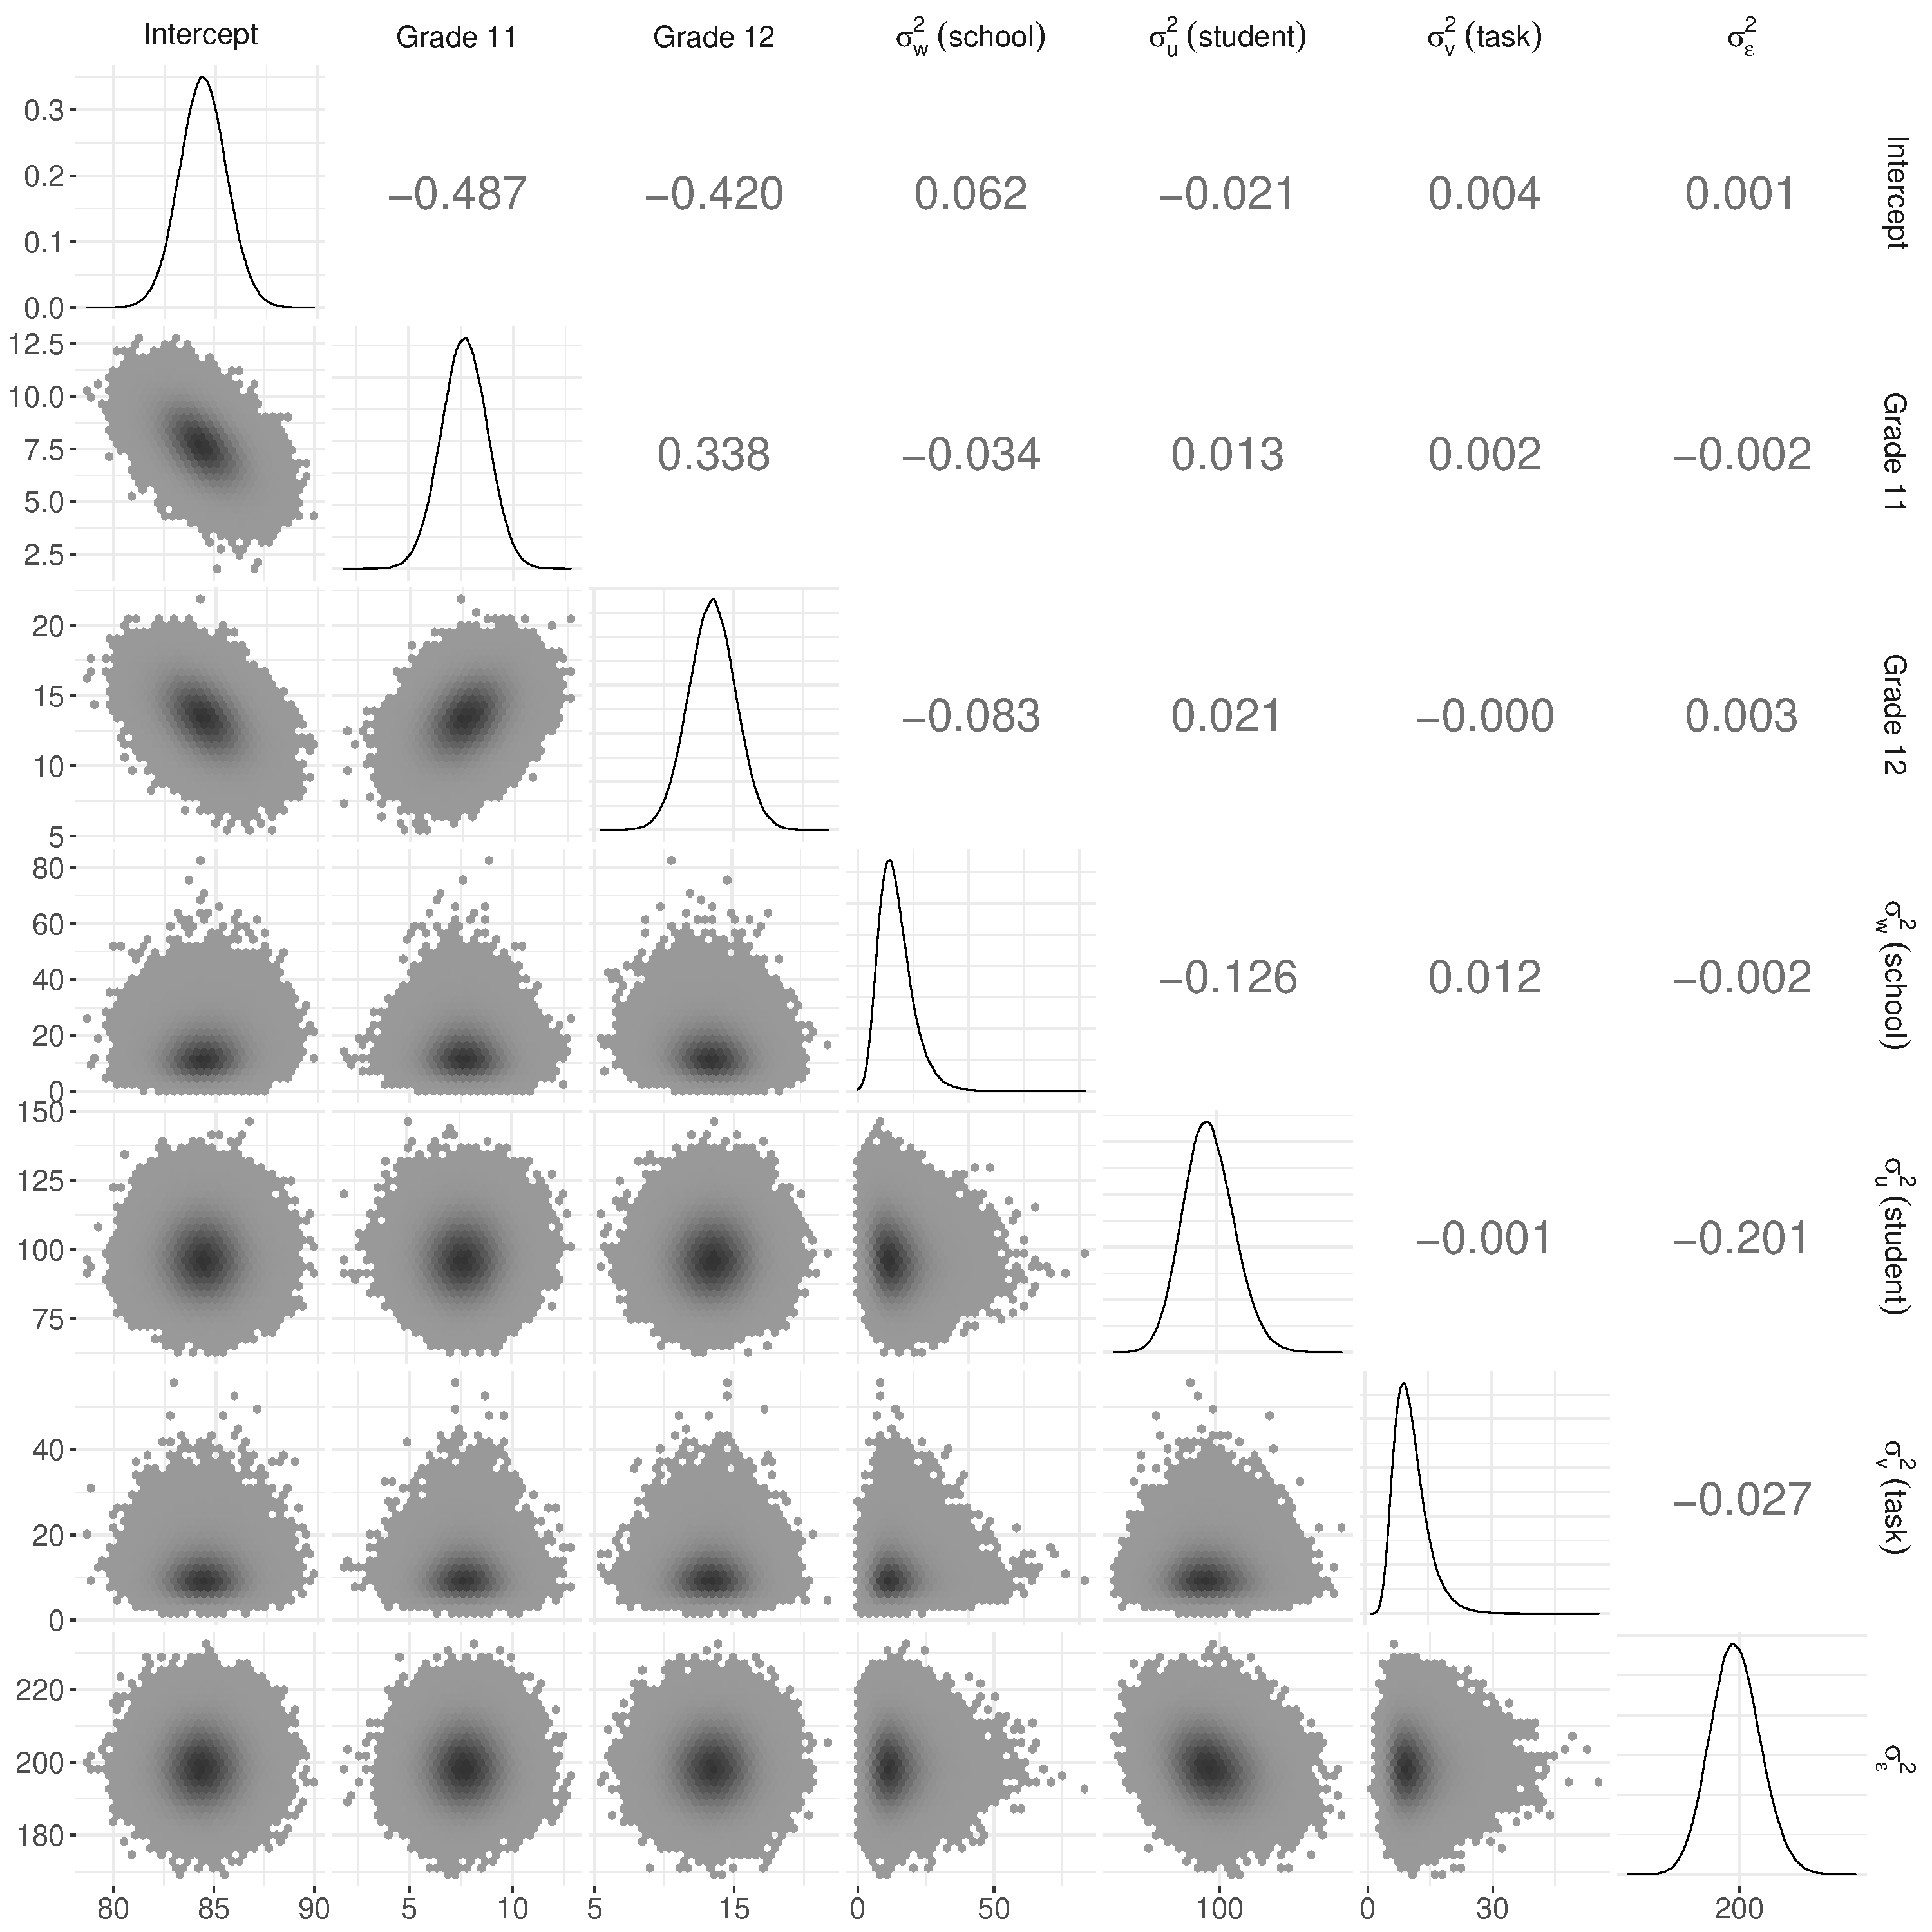
\includegraphics[width=\textwidth]{posteriorDescriptivesBaseline}
	\caption{A visual summary of the posterior distributions for the group level effects of the baseline data set. The strips above and right of the figures indicate the parameters compared. Figures on the diagonal show marginal density estimates. Figures below the diagonal show bivariate hexagonal histograms. The numbers above the diagonal indicate the Pearson correlation between the samples of the parameters.}
	\label{fig:baselinePosteriorDescriptives}
\end{figure}


\begin{figure}[!ht]
	\centering
	\begin{subfigure}{.5\textwidth}
		\centering
		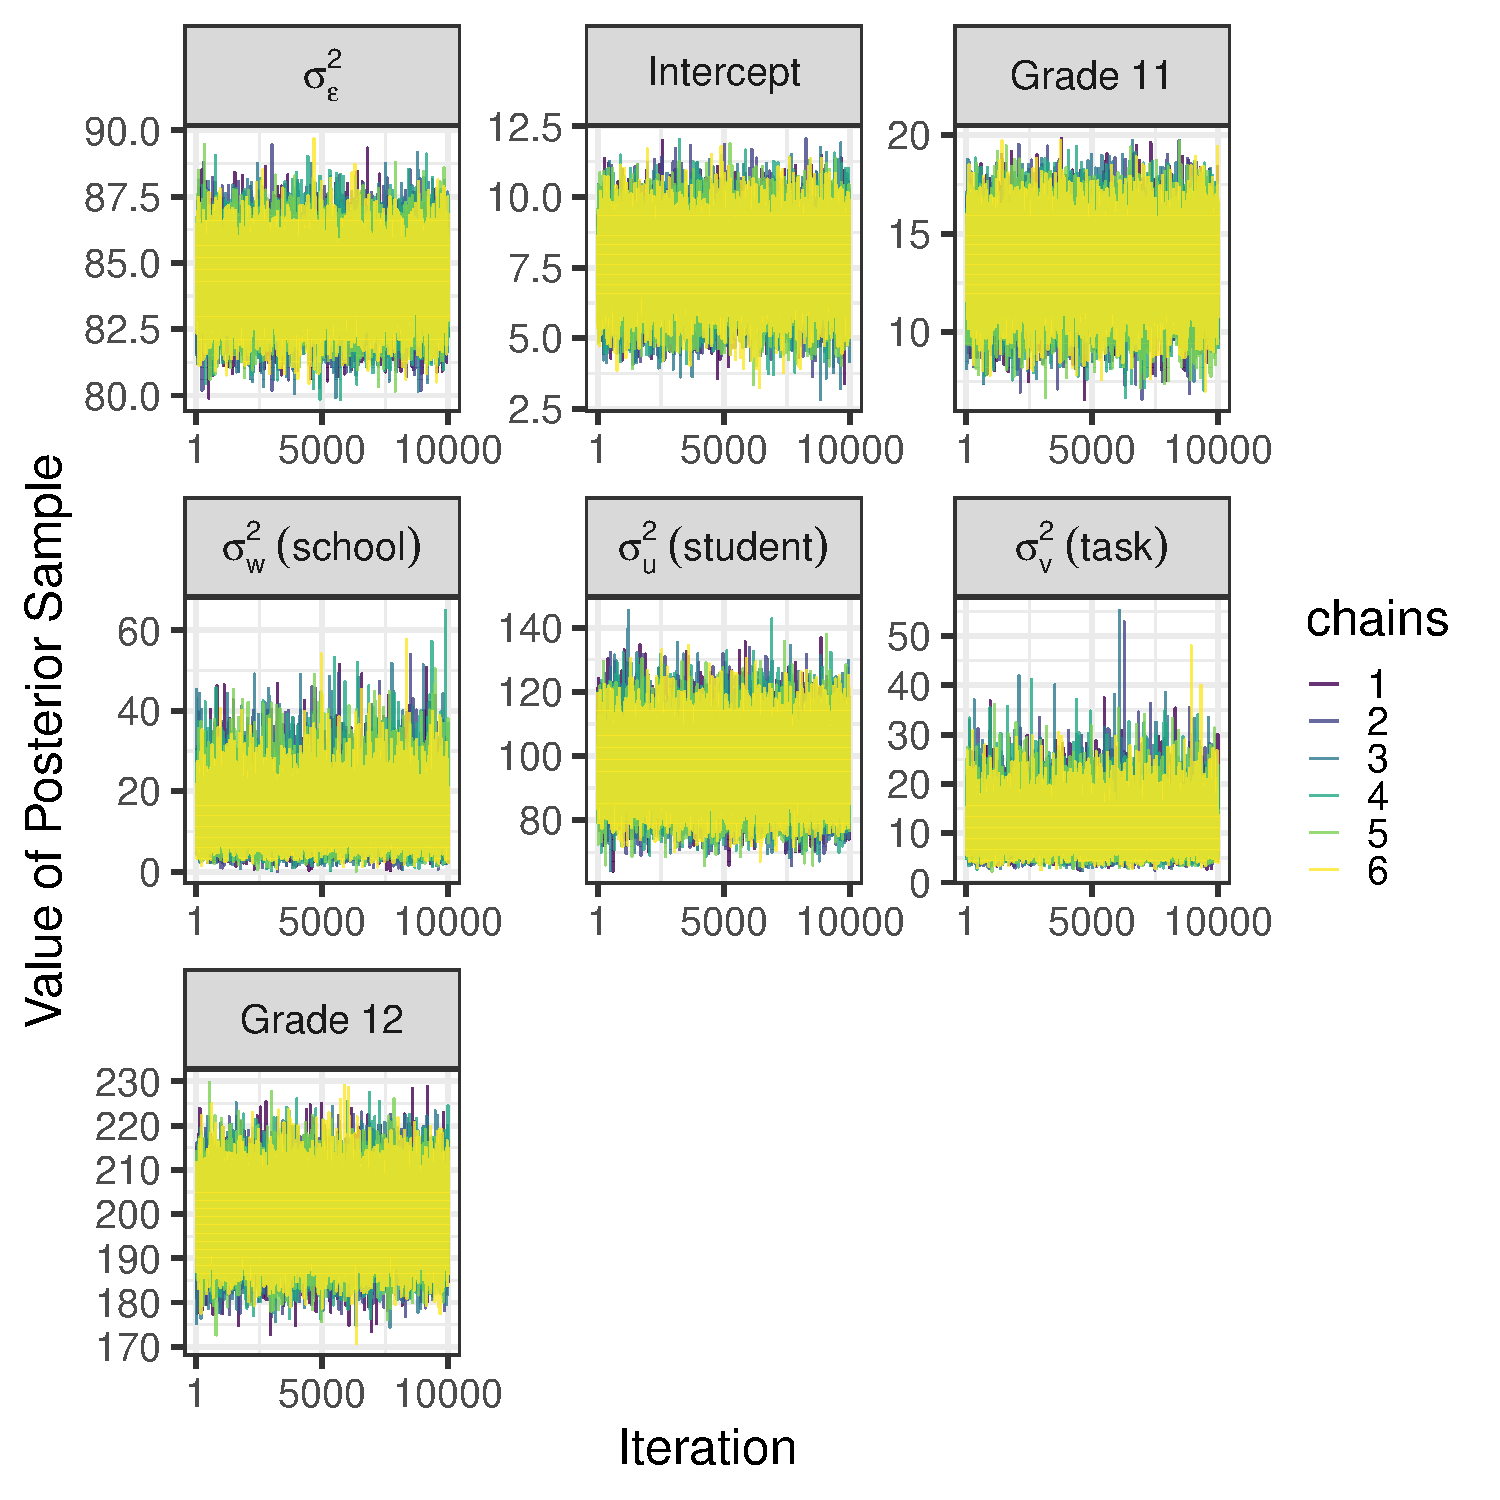
\includegraphics[width=\linewidth]{traceplotsBaseline}
	\end{subfigure}%
	\begin{subfigure}{.5\textwidth}
		\centering
		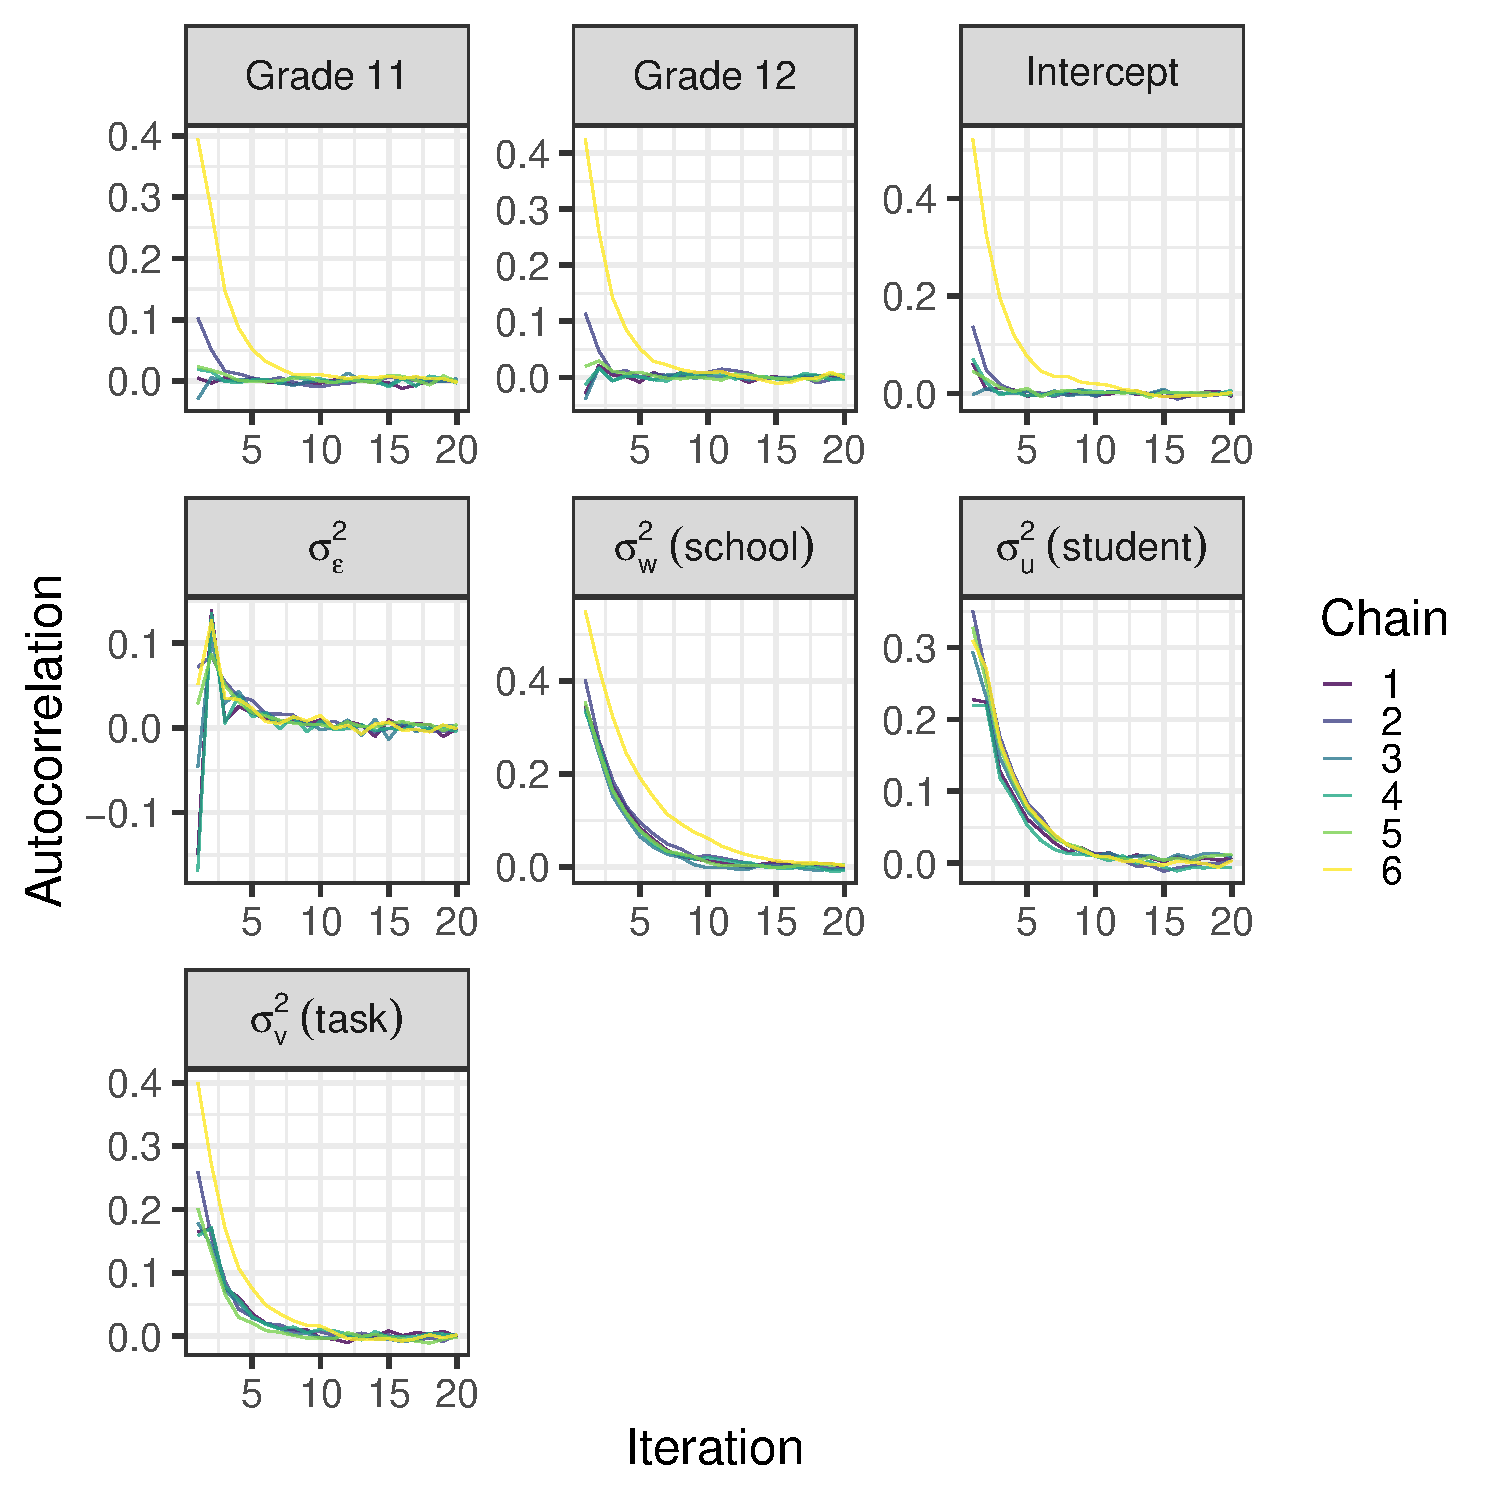
\includegraphics[width=\linewidth]{autocorrelationBaseline}
	\end{subfigure}%
	\caption{
		Convergence diagnostics for the analysis of the baseline data set. Left: trace plots of the first 10,000 posterior samples after warmup. The different chains appear indistinguishable, which indicates they converged. Right: Autocorrelation of the chains. The 0\textsuperscript{th} lag was omitted (as this is 1 by definition). The autocorrelation drops to 0 after about 5 iterations.}
	\label{fig:baselinePosteriorDiagnostics}
\end{figure}



\begin{figure}[!ht]
	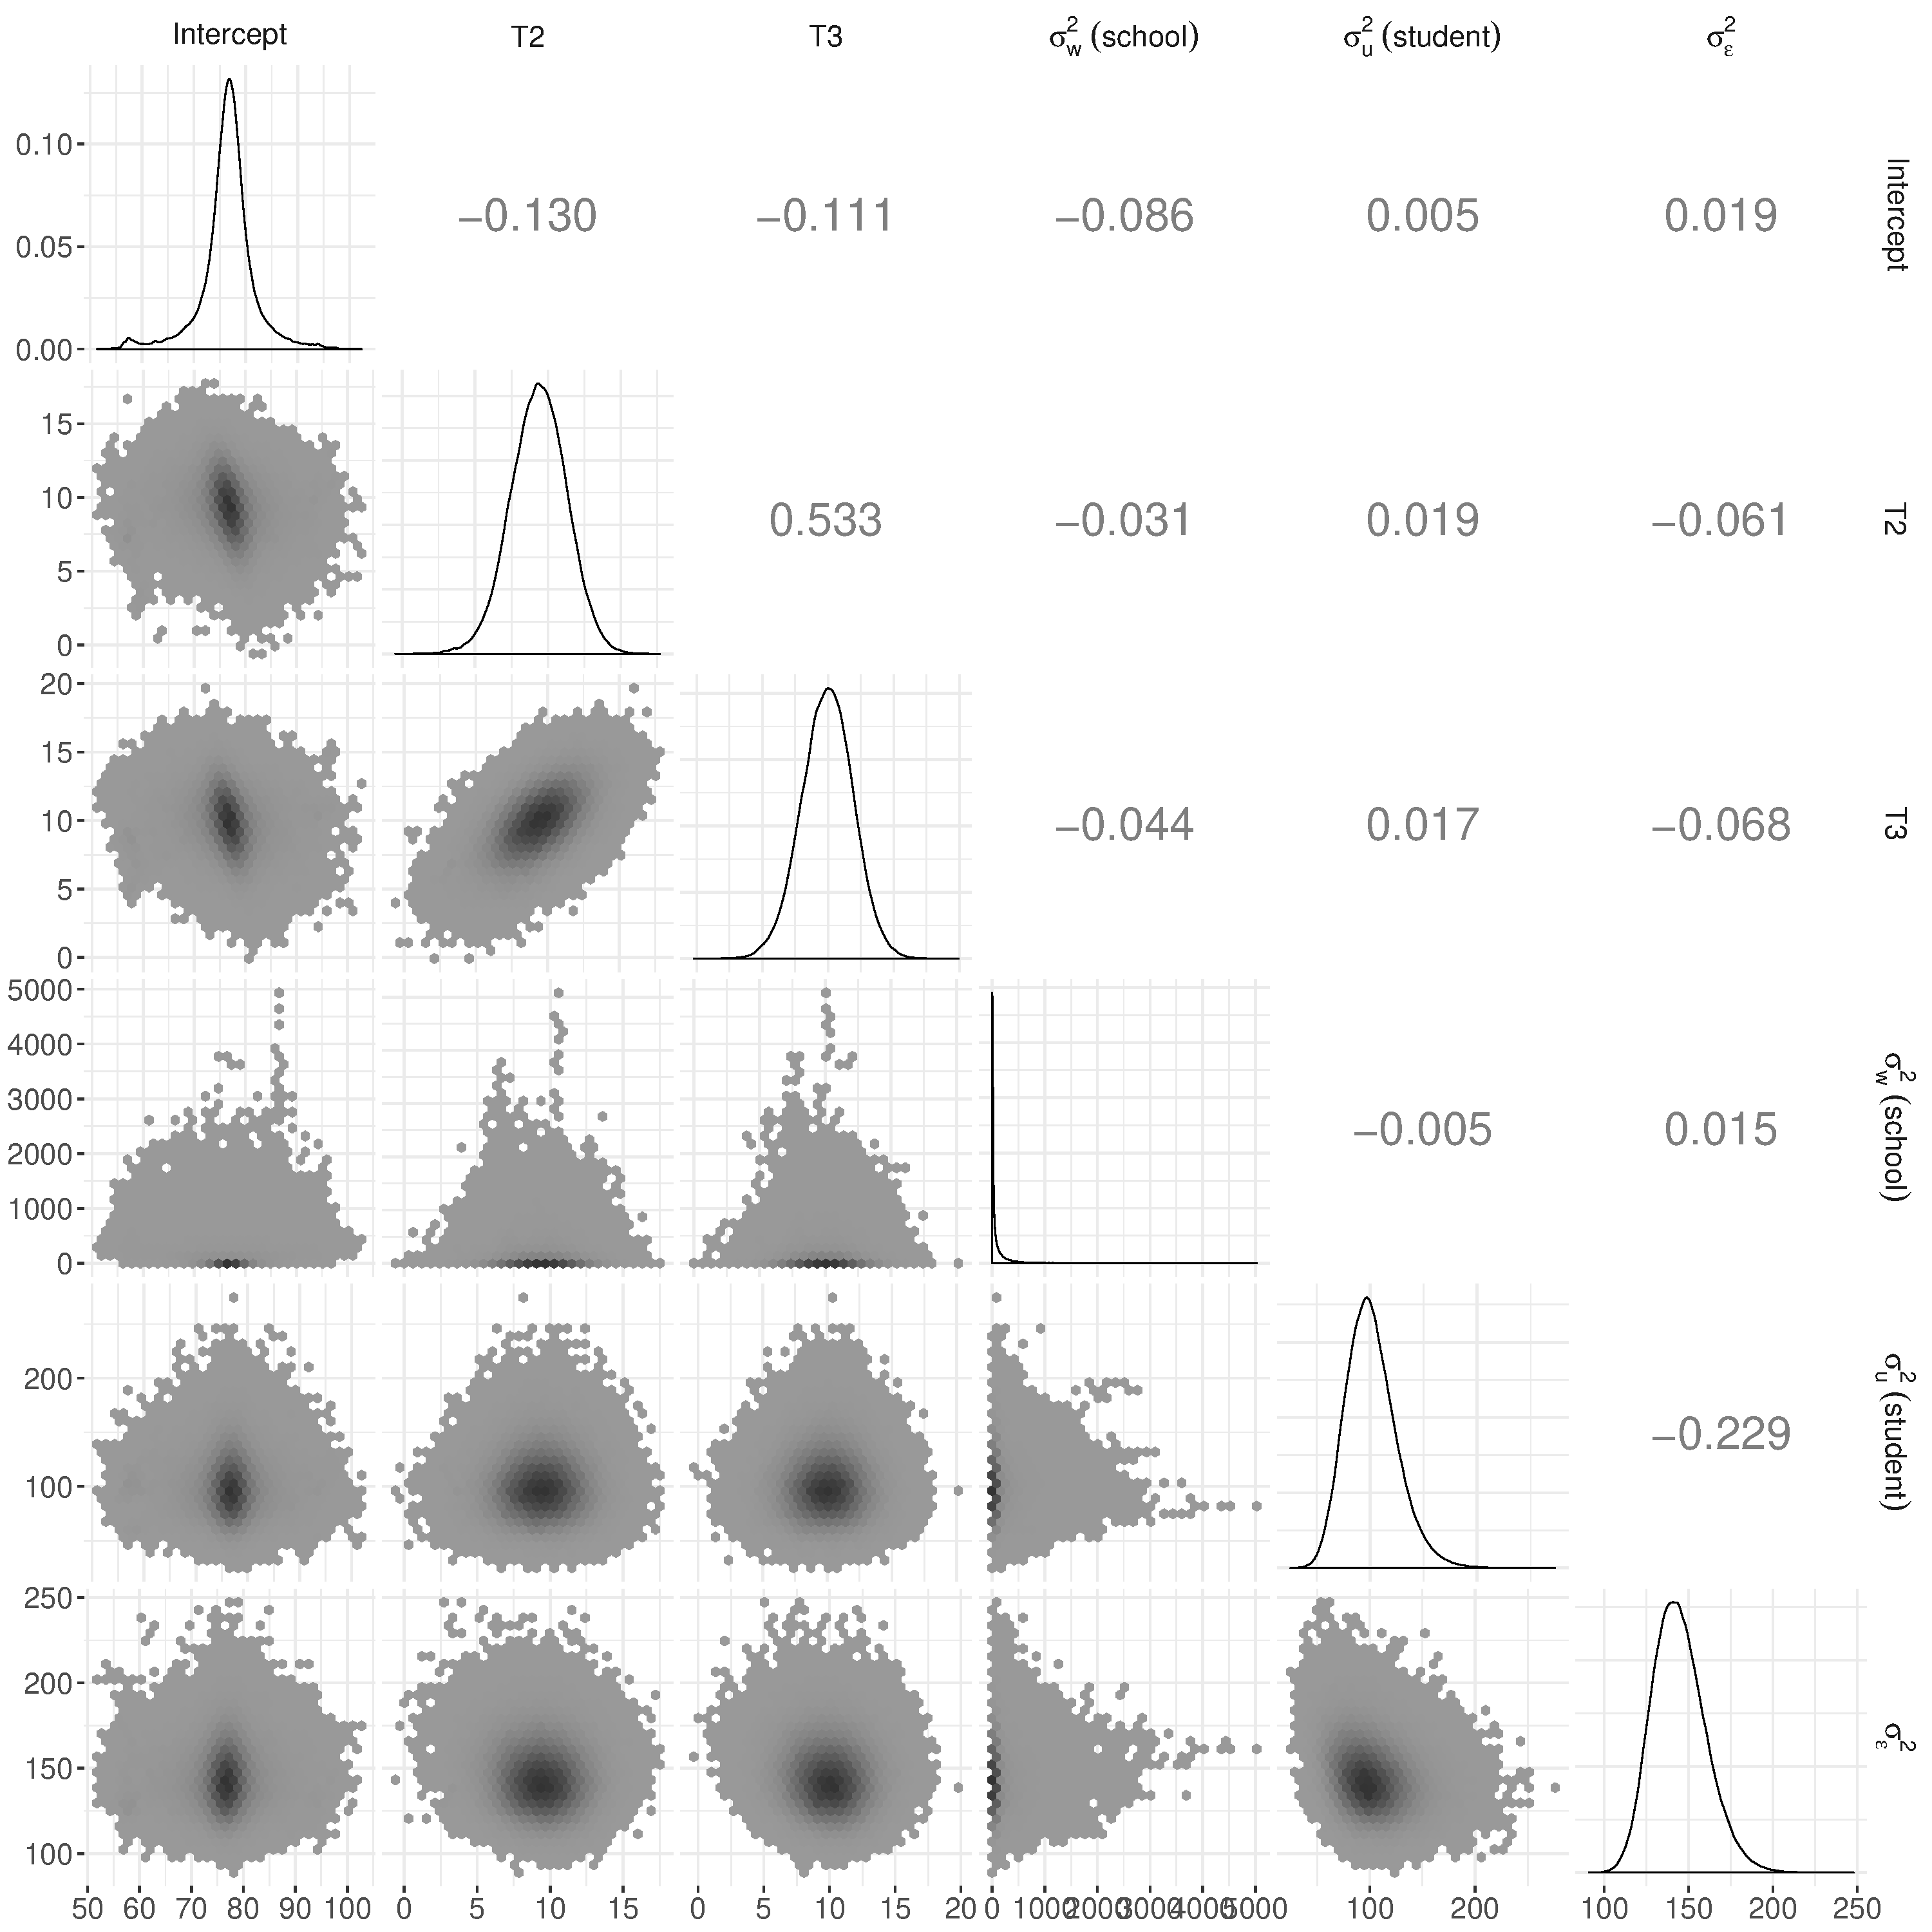
\includegraphics[width=\textwidth]{posteriorDescriptivesExperimental}
	\caption{A visual summary of the posterior distributions for the group level effects of the experimental data set. The strips above and right of the figures indicate the parameters compared. Figures on the diagonal show marginal density estimates. Figures below the diagonal show bivariate hexagonal histograms. The numbers above the diagonal indicate the Pearson correlation between the samples of the parameters.}
	\label{fig:productPosteriorDescriptives}
\end{figure}


\begin{figure}[!ht]
	\centering
	\begin{subfigure}{.5\textwidth}
		\centering
		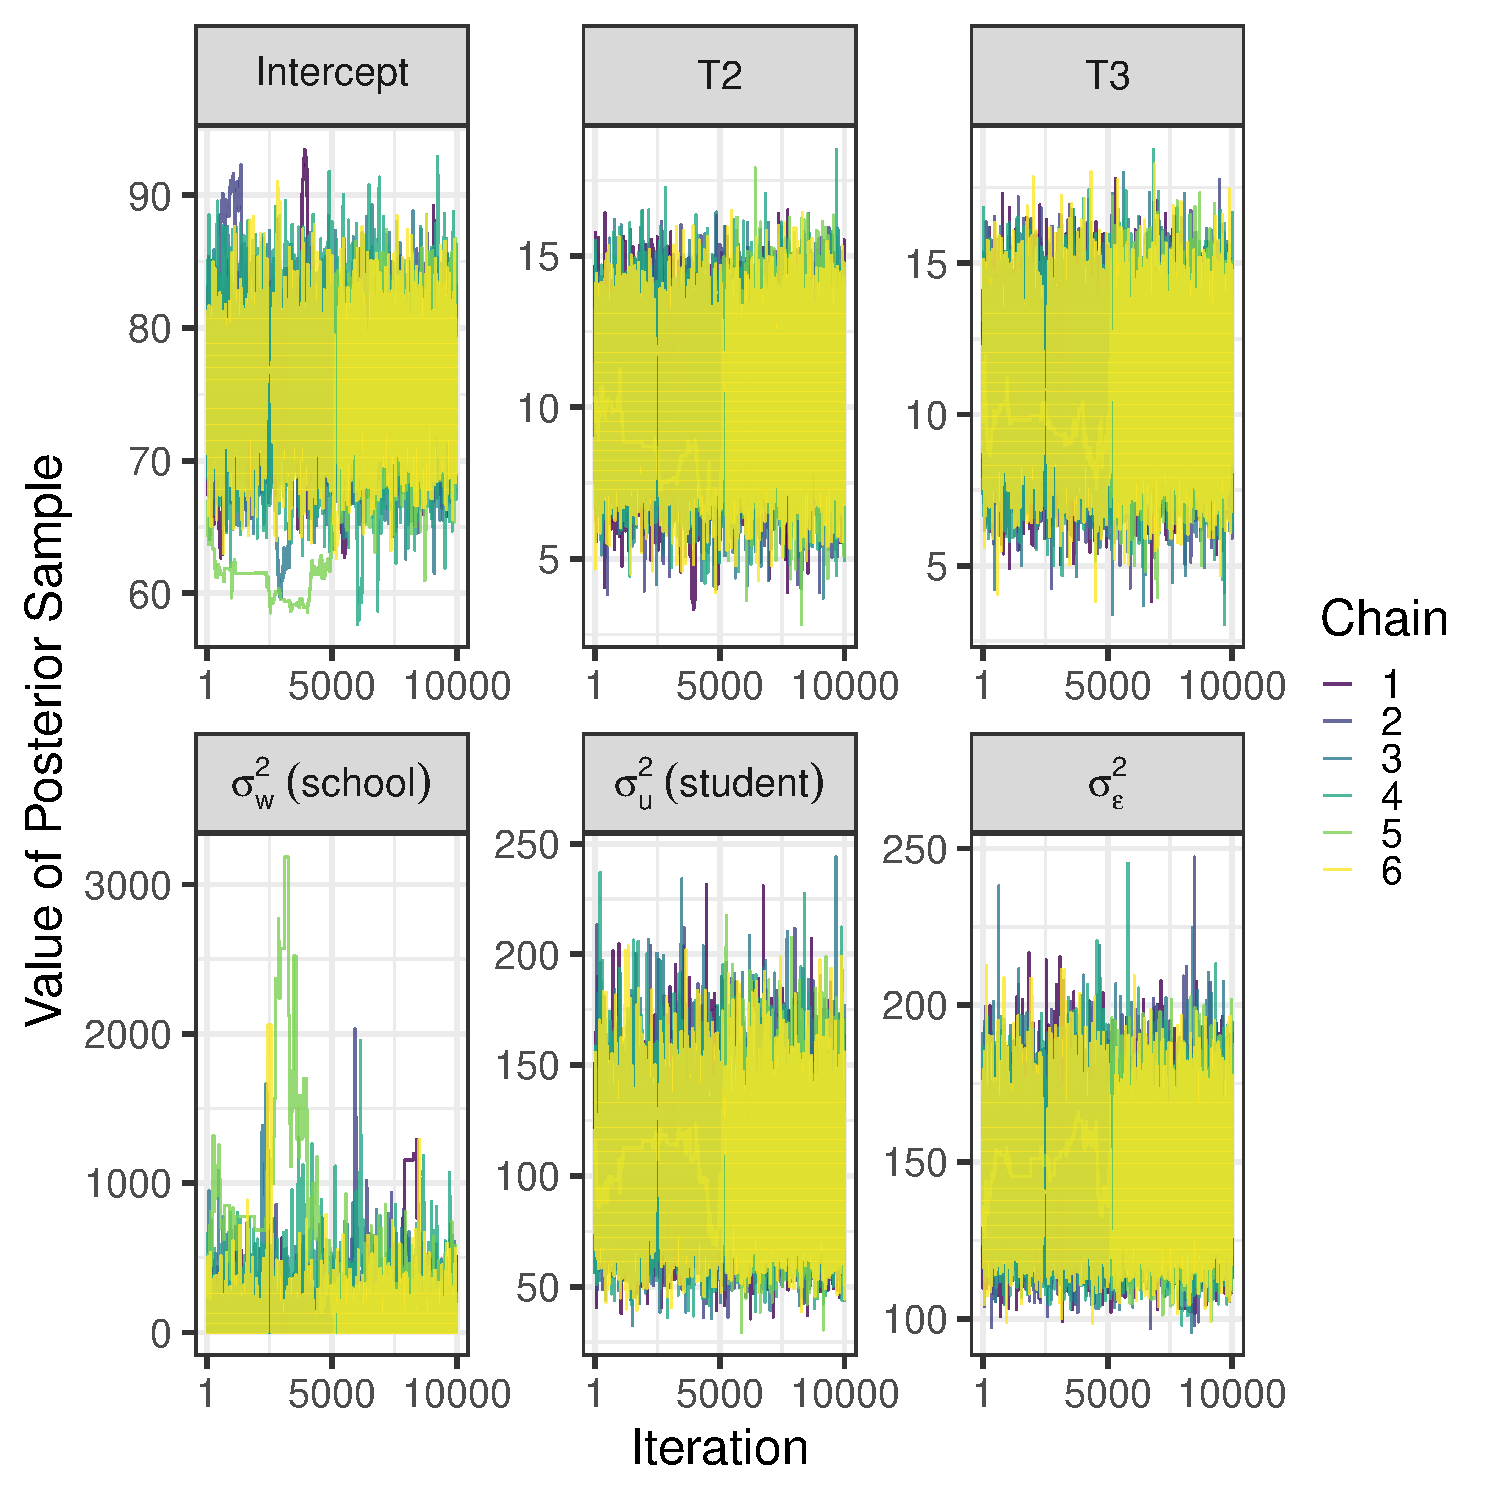
\includegraphics[width=\linewidth]{traceplotsExperimental.pdf}
	\end{subfigure}%
	\begin{subfigure}{.5\textwidth}
		\centering
		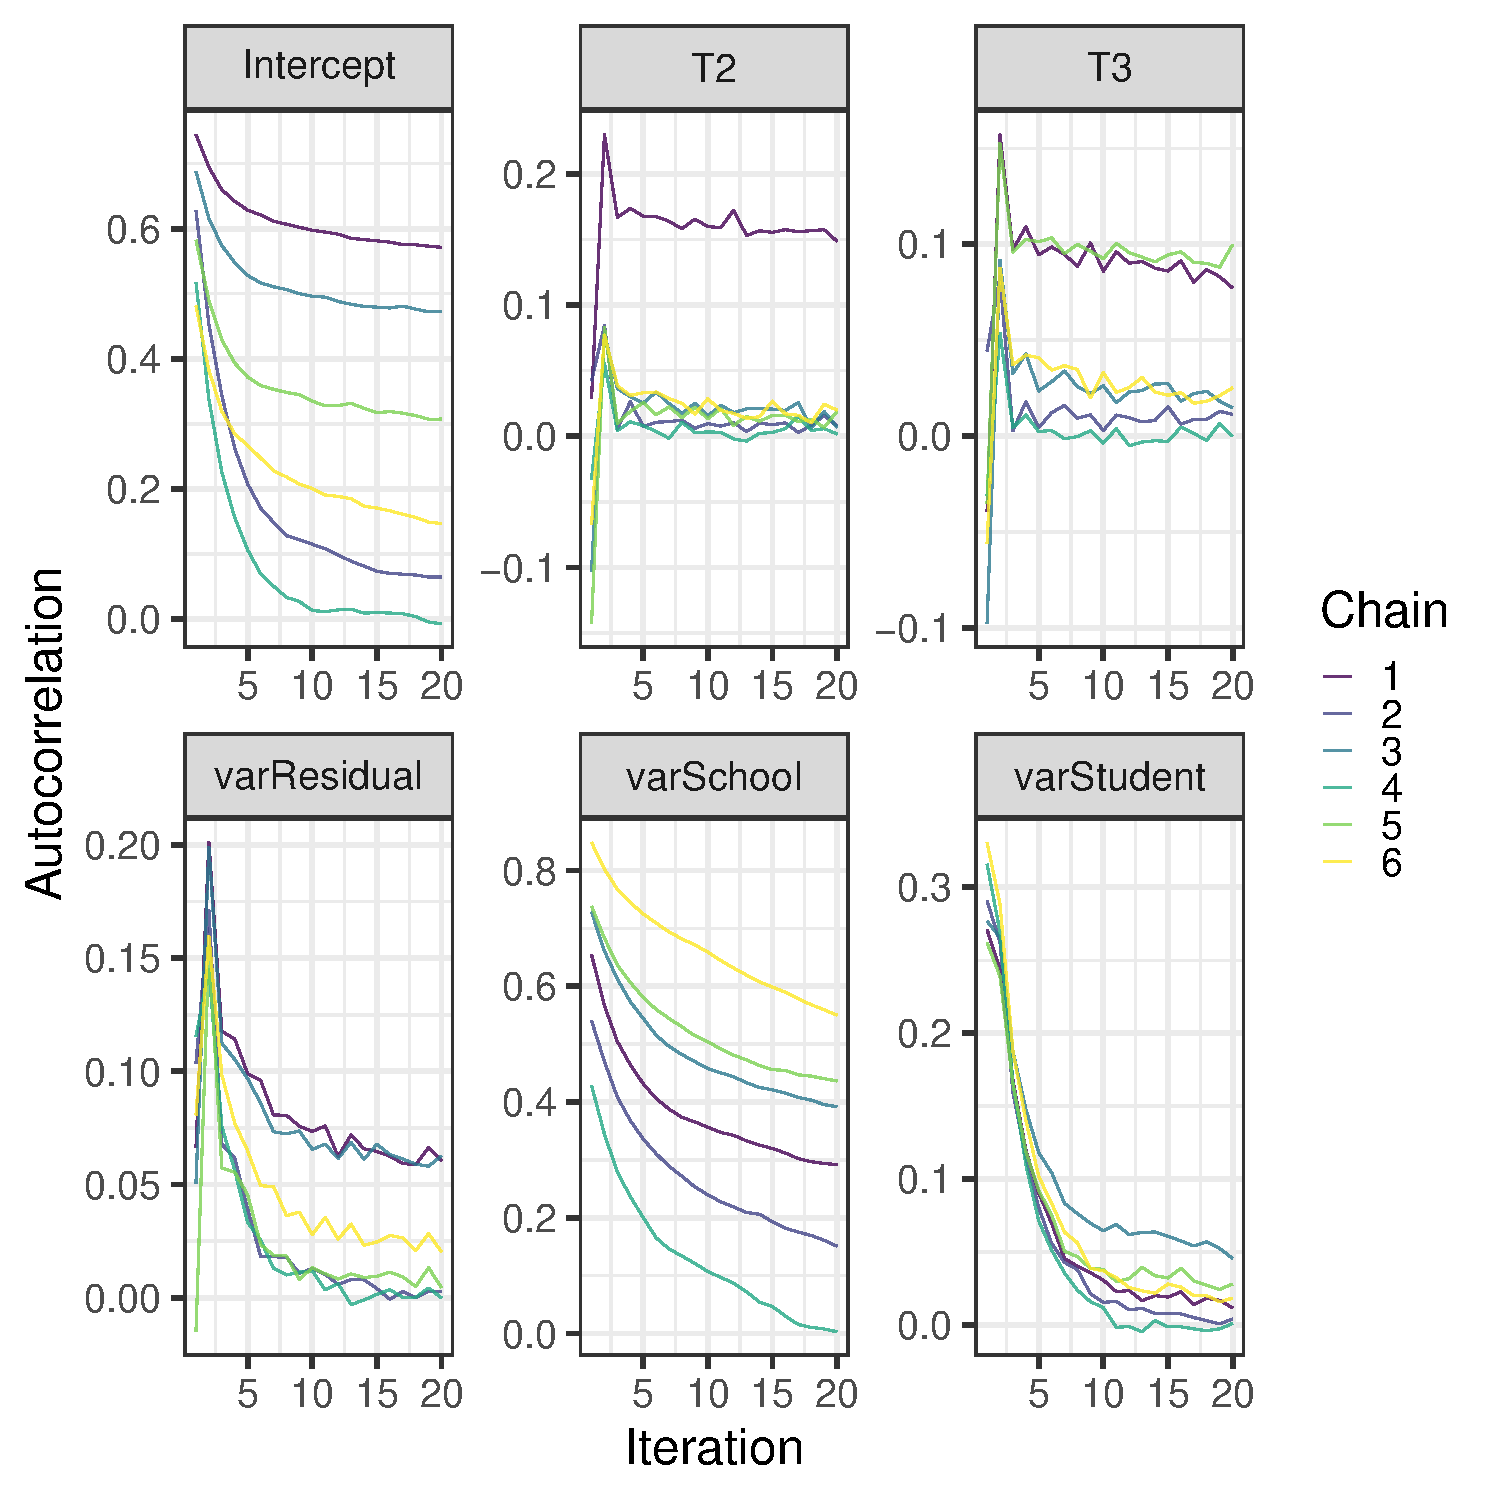
\includegraphics[width=\linewidth]{autocorrelationExperimental}
	\end{subfigure}%
	\caption{
		Convergence diagnostics for the analysis of the experimental data set.
		Left: trace plots of the first 10,000 posterior samples after warmup. The different chains appear indistinguishable, which indicates they converged. Right: Autocorrelation of the chains. The 0\textsuperscript{th} lag was omitted (as this is 1 by definition). The autocorrelation drops to 0 after about 5 iterations.}
	\label{fig:experimentalPosteriorDiagnostics}
\end{figure}



\end{document}

